\chapter{Experiments}
\label{c:experiments}
\IMRADlabel{results}



In this chapter we will present all environments we experimented with as well as \emph{hyper-experiments}, \ac{ie} experiments with the hyperparameters and their influence on the algorithm performance (in terms of the prediction error and similar metrics, not the computing time).

We split this chapter into two parts: Firstly, we will present the experiment setup we used and the different environments we tested on. Secondly, we present our results and put them in context of other results. All critical discussion and comparison with related work will take place in~\autoref{c:discussion}.

\section{Setup}
	In this section we will introduce the experiment setup and all the different environments we used for evaluation.

	\subsection{Environments}
		This section covers the different environments we used and changed we might have applied to them. Do generate the data, you have to run the file \texttt{src/data.py} with the desired experiment ID as the first argument, \ac{eg} \texttt{python src/data.py pendulum\_damped}. If no argument is given, a regeneration of the data from all experiments is triggered. For each of the following environments we summarize the most important data about the environment at the start of the subsection, including the experiment ID.

		\subsubsection{Proof-of-Concept: Classic LGDS}
			\begin{itemize}
				\item Experiment ID: \texttt{lgds}
			\end{itemize}

			As a proof-of-concept and to empirically verify our proof on the exactness of the cubature rule and hence the similar expected performance for plain linear systems, we benchmark our algorithm against a simple linear system. The linear system has a two-dimensional state \( \vec{y} \coloneqq \begin{bmatrix} x_1 & x_2 \end{bmatrix}^T \) with the dynamics
			\begin{align*}
				\dot{x}_1 &= x_2 \\
				\dot{x}_2 &= -x_1
			\end{align*}
			The initial state \( \vec{s}_1 \) is sampled from a Gaussian with mean \( \begin{bmatrix} 0.1 & 0.2 \end{bmatrix}^T \) and covariance \( \diag\big(10^{-5}, 10^{-5}\big) \). The system is integrated using the implicit Runge-Kutta Radau~IIA~\cite{guglielmiImplementingRadauIIA2001} method with an evaluation interval of \( h = 0.1 \) for \( T = 240 \) time steps where only the first \( T_\train = 120 \) steps are used for training and the remaining \(120\) are used for validation. The raw data is shown in~\autoref{fig:envLgds}.

			As the system's eigenvalues \( -i \), \( i \) are purely imaginary, the integrated system rings around the equilibrium \( \begin{bmatrix} 0 & 0 \end{bmatrix}^T \) infinitely.

			\begin{figure}
				\centering
				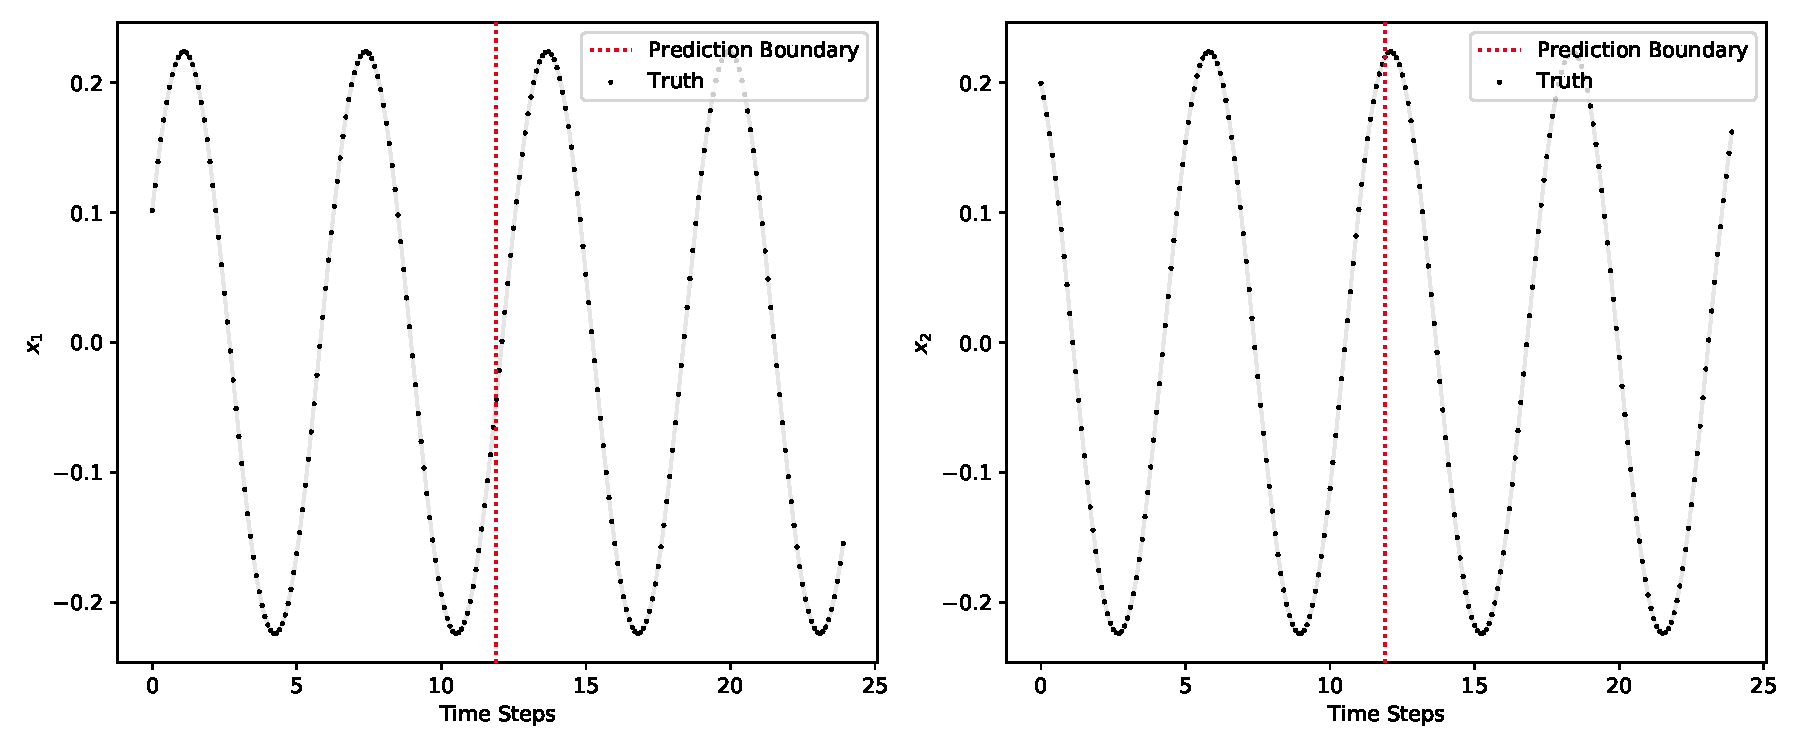
\includegraphics[width=\linewidth]{figures/experiments/environments/observations-lgds-N0.pdf}
				\caption{Plot of the raw data used for training the proof-of-concept \ac{lgds} environment. The black dots represent the actual data points, all before the red prediction boundary are used for training, the rest for validation. The faint gray line emphasizes the connection between the data points and that they are actually generated from a dynamical system.}
				\label{fig:envLgds}
			\end{figure}
		% end

		\subsubsection{(Damped) Pendulum}
			\begin{itemize}
				\item Experiment ID: \texttt{pendulum} and \texttt{pendulum\_damped}
			\end{itemize}

			The first nonlinear system we look at is the (inverted) pendulum in both an undamped and a damped setting. For this experiment, we use the angular state \( \vec{y} = \begin{bmatrix} \theta & \dot{\theta} \end{bmatrix} \) where \(\theta\) is the displacement angle (see~\autoref{fig:envPendulumSketch}). The dynamics are specified by the \ac{ode}
			\begin{equation*}
				\ddot{\theta} = \sin\theta - d \dot{\theta}
			\end{equation*}
			that is solved using the Radau~IIA~\cite{guglielmiImplementingRadauIIA2001} \ac{ivp} integrator (after transforming the \ac{ode} in a first-order \ac{ode} system). The initial velocity is set to \(0\) and the initial position is sampled from a Gaussian with mean \( \pi/36 \) and variance \( \pi/8 \). This puts the pendulum in motion as it falls down from its initial position. For the undamped pendulum, we set \( d = 0 \). For both environments, we use an evaluation interval of \( h = 0.1 \) for \( T = 1000 \) time steps where only the first \( T_\train = 500 \) steps are used for training and the remaining \(500\) are used for validation. The raw data is shown in~\autoref{fig:envPendulum} for the undamped and~\autoref{fig:envPendulumDamped} for the damped pendulum.

			The damped pendulum is especially interesting as the system looses energy (\ac{ie} the sum of the kinetic and potential energy decreases over time) and the embedding has to encode this behavior.

			\begin{figure}
				\centering
				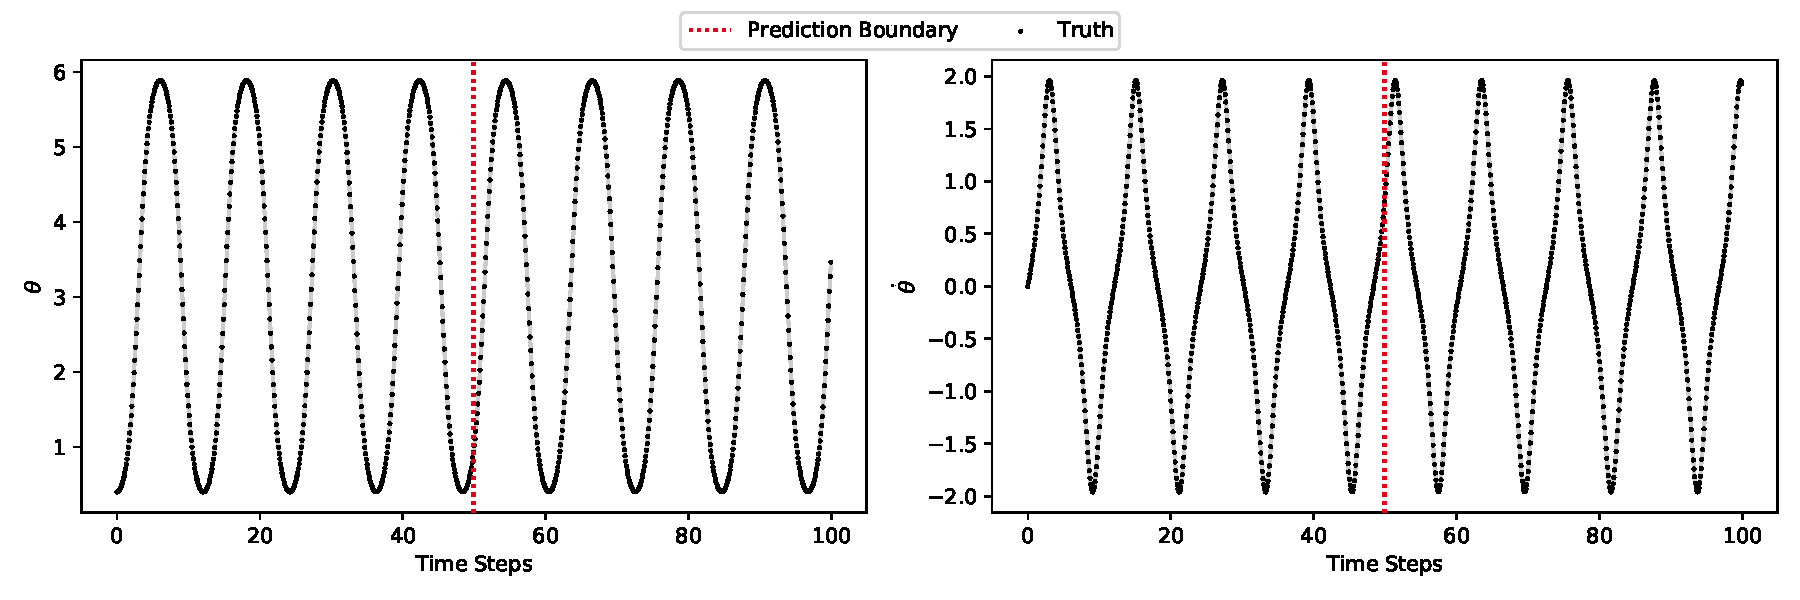
\includegraphics[width=\linewidth]{figures/experiments/environments/observations-pendulum-N0.pdf}
				\caption{Plot of the raw data used for training the undamped pendulum environment. The left plot shows the displacement and the right plot the angular velocity. The black dots represent the actual data points, all before the red prediction boundary are used for training, the rest for validation. The faint gray line emphasizes the connection between the data points and that they are actually generated from a dynamical system.}
				\label{fig:envPendulum}
			\end{figure}
			\begin{figure}
				\centering
				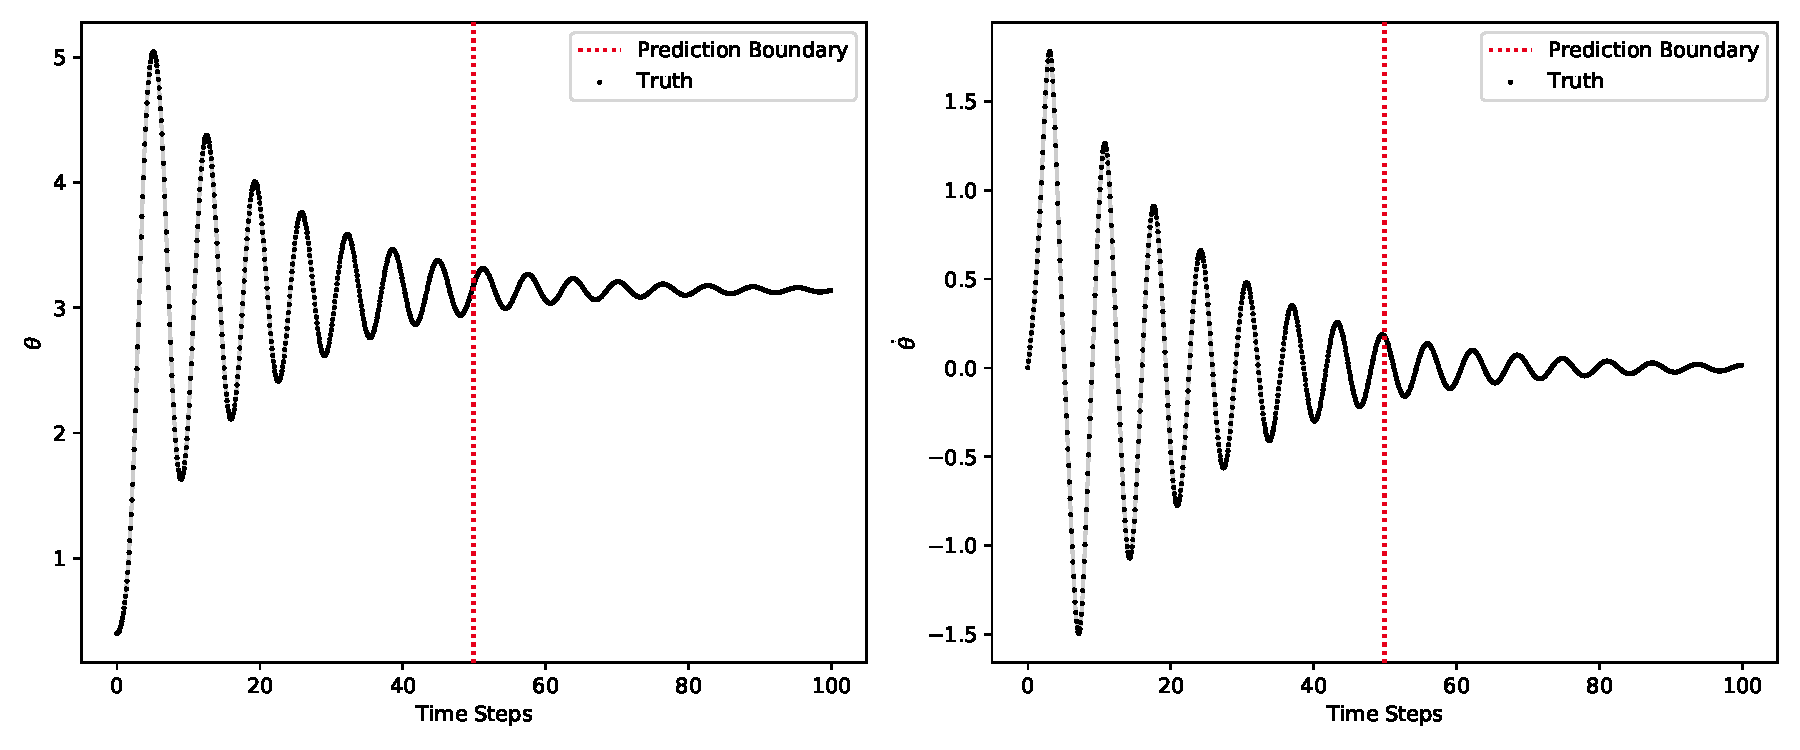
\includegraphics[width=\linewidth]{figures/experiments/environments/observations-pendulum-damped-N0.pdf}
				\caption{Plot of the raw data used for training the damped pendulum environment. The left plot shows the displacement and the right plot the angular velocity. The black dots represent the actual data points, all before the red prediction boundary are used for training, the rest for validation. The faint gray line emphasizes the connection between the data points and that they are actually generated from a dynamical system.}
				\label{fig:envPendulumDamped}
			\end{figure}

			\begin{figure}
				\centering
				\tikzSimplePendulum
				\caption{Illustration of the pendulum environment. The pendulum has length \(L\) and mass \(m\) and is attached to a fixed point in the center around which it can swing. In the case of the undamped pendulum, it swings freely, otherwise it is damped with a damping constant \(d\).}
				\label{fig:envPendulumSketch}
			\end{figure}
		% end

		\subsubsection{Gym Pendulum}
			\begin{itemize}
				\item Experiment ID: \texttt{pendulum\_gym}
			\end{itemize}

			This is a sine/cosine version of the pendulum introduced before, but without damping. We use the environment of OpenAI Gym~\cite{brockmanOpenAIGym2016} for generating the data used for training. The motion equations are still the same as for the non-Gym pendulum
			\begin{equation*}
				\ddot{\theta} = \sin\theta
			\end{equation*}
			with \( d = 0 \) as the Gym pendulum does not include damping, but the state is defined as the sine and cosine of the angle:
			\begin{equation*}
				\vec{y} \coloneqq
					\begin{bmatrix}
						\cos\theta \\
						\sin\theta \\
						\dot{\theta}
					\end{bmatrix}
			\end{equation*}
			The Gym environment uses the Euler method for integrating the \ac{ode} with a step size of \( h = 0.05 \). We generate \( T = 100 \) time steps of which \( T_\train = 50 \) are used for training and the other \(50\) for validation. The raw data is shown in~\autoref{fig:envPendulumGym}.

			\begin{figure}
				\centering
				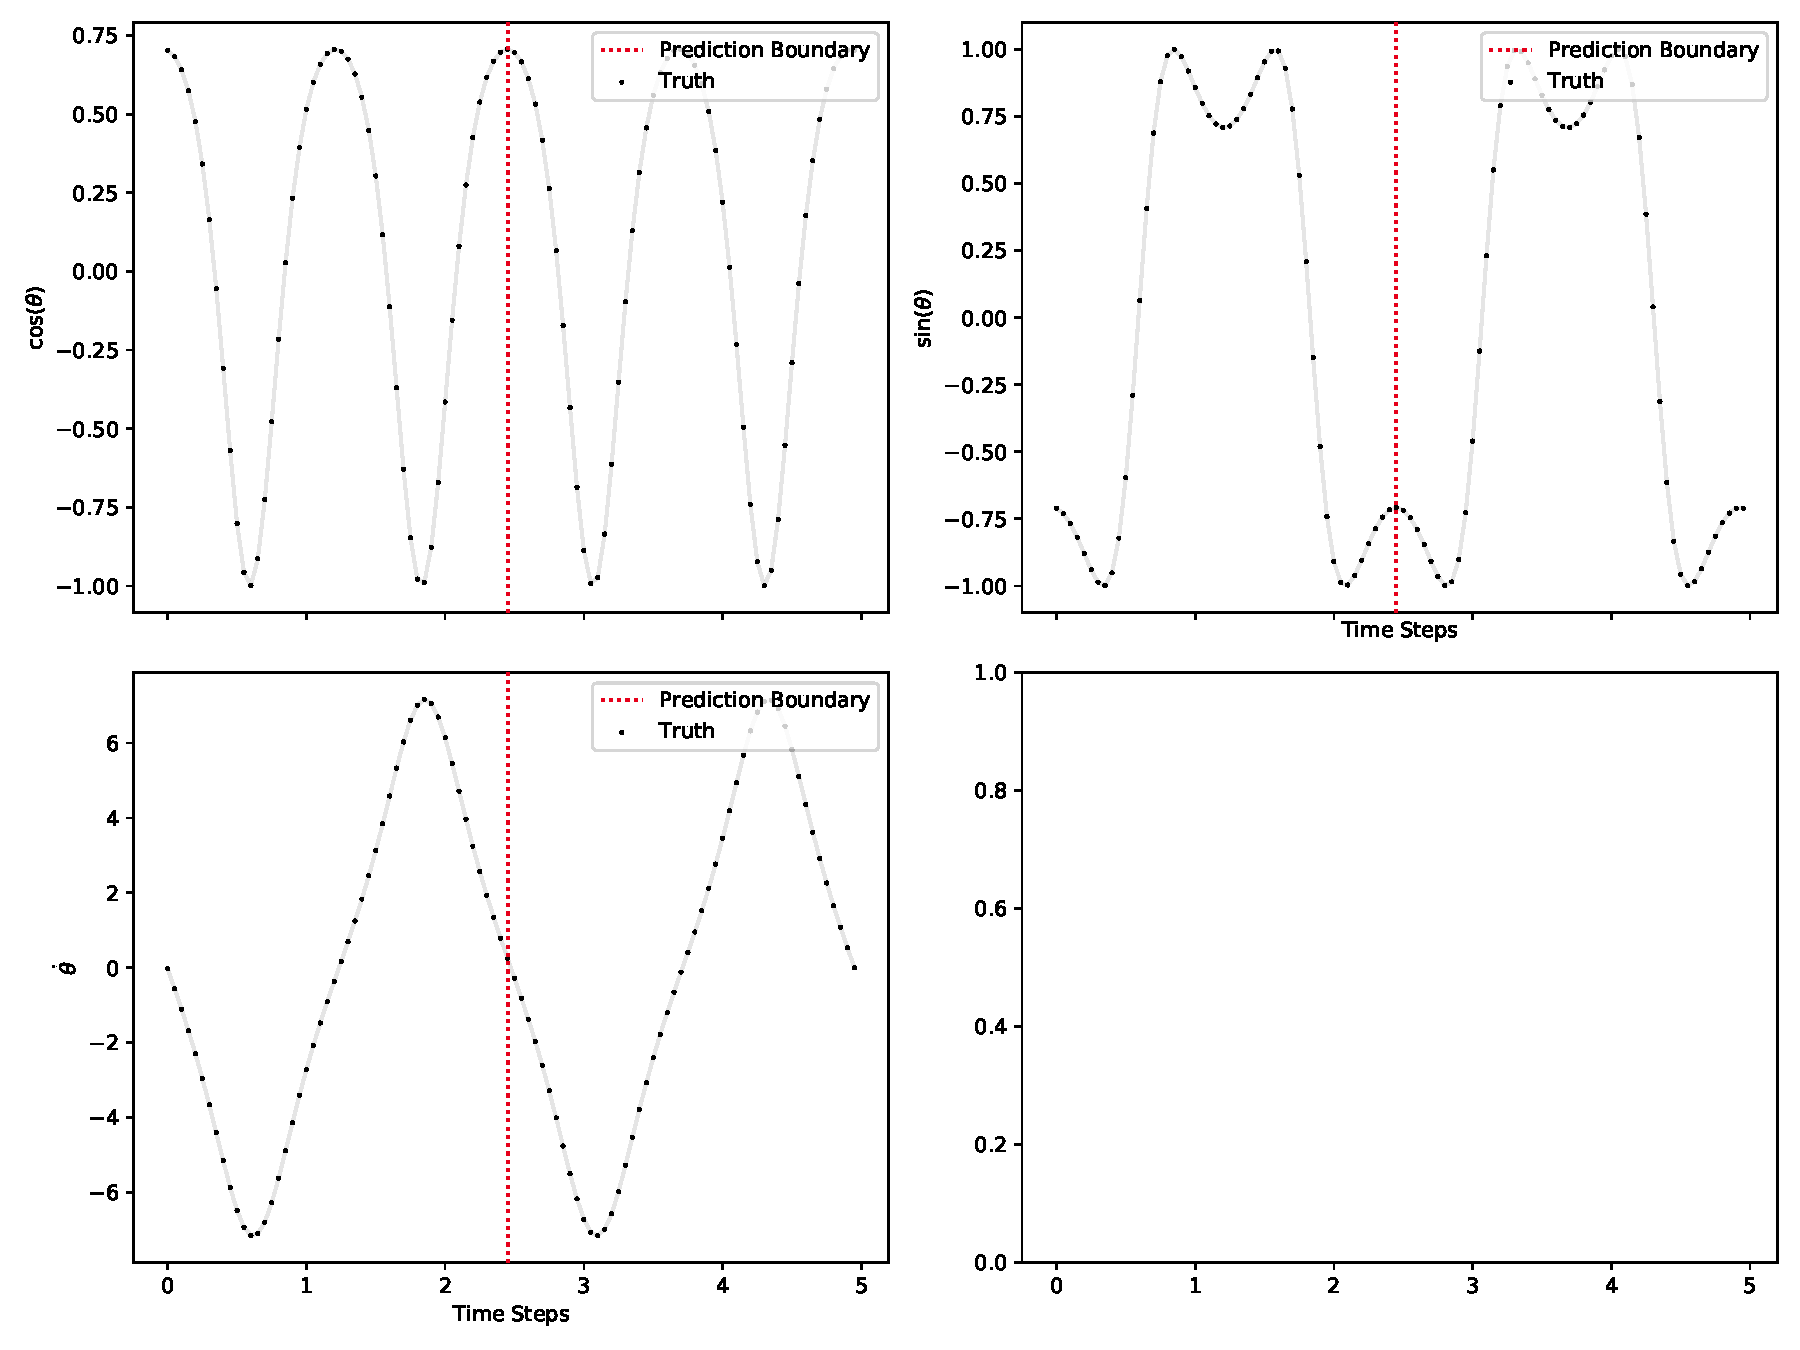
\includegraphics[width=\linewidth]{figures/experiments/environments/observations-pendulum-gym-N0.pdf}
				\caption{Plot of the raw data used for training the Gym pendulum environment. The top row shows the cosine/sine of the displacement of the pendulum and the bottom plot shows the angular velocity. The black dots represent the actual data points, all before the red prediction boundary are used for training, the rest for validation. The faint gray line emphasizes the connection between the data points and that they are actually generated from a dynamical system.}
				\label{fig:envPendulumGym}
			\end{figure}
		% end

		\subsubsection{Gym Cartpole}
			\label{subsubsec:cartpole}

			\begin{itemize}
				\item Experiment ID: \texttt{cartpole\_gym}
			\end{itemize}

			The second last environment we run experiment on is the cartpole environment. In the cartpole environment, an inverted pendulum is build on a (typically controlled, but otherwise freely movable) cart. If the pendulum falls town, the torque on the joint is translated into a force moving the cart around. This creates nonlinear coupling and therefore highly nonlinear dynamics. A sketch of the cartpole environment is given in~\autoref{fig:envCartpoleGymSketch}. As for the previous pendulum, we rely on the cartpole implementation of Gym. We slightly modified the environment to be uncontrolled, as the environment usually has discrete actions for pushing the cart left or right. This modification is shown in~\autoref{lst:uncontrolledCartPole}. The state of the environment is given as
			\begin{equation*}
				\vec{y} \coloneqq
					\begin{bmatrix}
						x \\
						\dot{x} \\
						\theta \\
						\dot{\theta}
					\end{bmatrix}
			\end{equation*}
			where \(x\) is the cart position, \(\dot{x}\) is the cart velocity, \(\theta\) is the pole angle and \(\dot{\theta}\) is the angular velocity. The implemented equations of movement, taken from~\cite{florianCorrectEquationsDynamics2005}, are given as
			\begin{align*}
				\ddot{\theta} &= \frac{g \sin\theta + \cos\theta \Big(\! \frac{-F - m_p \ell \dot{\theta}^2 \sin\theta}{m_c + m_p} \!\Big)}{\ell \Big(\! \frac{4}{3} - \frac{m_p \cos^2\theta}{m_c + m_p} \!\Big)} \\
				\ddot{x} &= \frac{F + m_p \ell \big( \dot{\theta}^2 \sin\theta - \ddot{\theta} \cos\theta \big)}{m_c + m_p}
			\end{align*}
			where \( g = \SI{9.81}{\meter\per\second\squared} \) is the gravitational acceleration, \( m_p = \SI{0.1}{\kilogram} \) and \( m_c = \SI{1}{\kilogram} \) are the masses of the pole and cart, respectively, \( 2\ell = \SI{1}{\meter} \) is the pole length and \( [F] = \si{\newton} \) is the external (control) force acting on the cart that we set to \( \SI{0}{\newton} \). The Gym environment uses an implicit Euler method\footnote{As we already said in~\autoref{subsubsec:integrationProblems}, this has to be set manually with \lstinline|env.kinematics_integrator = 'implicit-euler'|.} for integrating the \ac{ode} with a step size of \( h = 0.02 \). We generate \( T = 300 \) time steps of which we use \( T_\train = 150 \) for training and the remaining \(150\) steps for validation. The raw data is shown in~\autoref{fig:envCartpoleGym}.

			\begin{lstlisting}[caption={Modification of Gym's cartpole environment to get an uncontrolled cartpole.}, label=lst:uncontrolledCartPole]
from gym.envs.classic_control import CartPoleEnv

class UncontrolledCartPole(CartPoleEnv):
	def __init__(self):
	super().__init__()

	self.force_mag = 0.0
			\end{lstlisting}

			\begin{figure}
				\centering
				\tikzCartpole
				\caption{Illustration of the cartpole environment. The cart has mass \(m_c\), the pole \(m_p\) with length \(L\). The cart can move freely on the \(x\) axis, while the pendulum can swing freely around the center of the cart, causing it to move.}
				\label{fig:envCartpoleGymSketch}
			\end{figure}

			\begin{figure}
				\centering
				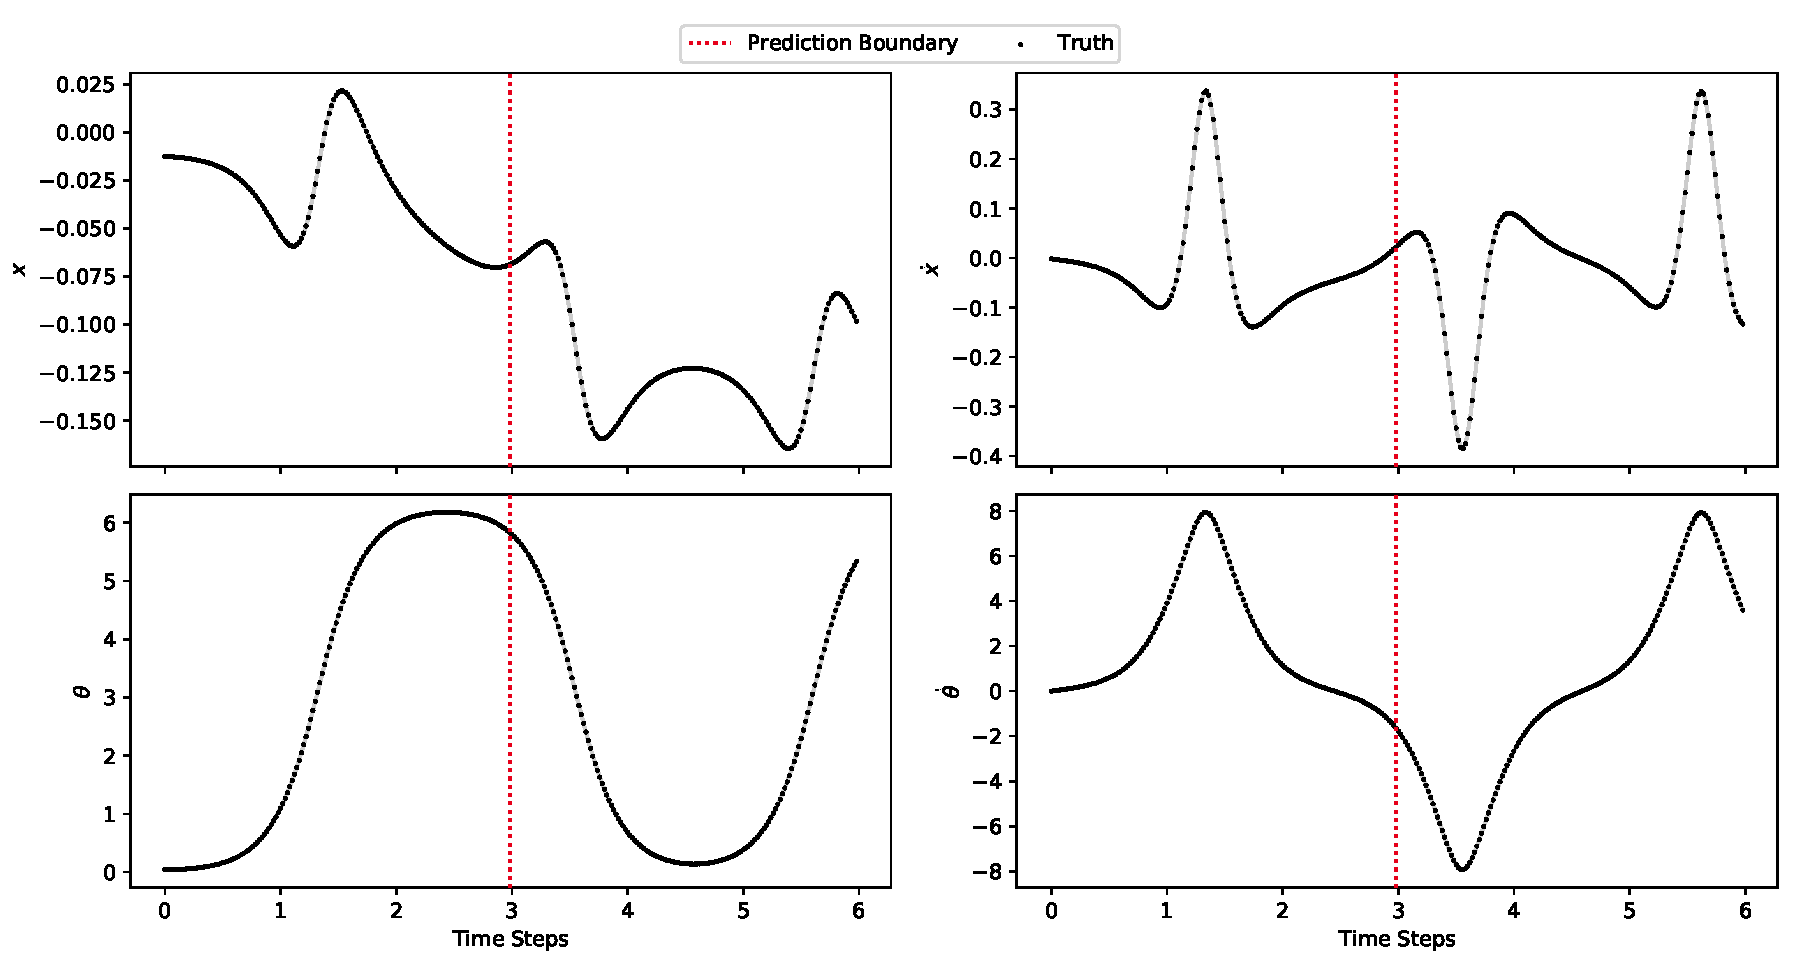
\includegraphics[width=\linewidth]{figures/experiments/environments/observations-cartpole-gym-N0.pdf}
				\caption{Plot of the raw data used for training the Gym cartpole environment. The top plot is the cart position (left) and velocity (right), the row the pole displacement (left) and angular velocity (right). The black dots represent the actual data points, all before the red prediction boundary are used for training, the rest for validation. The faint gray line emphasizes the connection between the data points and that they are actually generated from a dynamical system.}
				\label{fig:envCartpoleGym}
			\end{figure}
		% end

		\subsubsection{Gym Double Pendulum}
			\begin{itemize}
				\item Experiment ID: \texttt{acrobot\_gym}
			\end{itemize}

			The last environment we test is the double pendulum, implemented in Gym as the \emph{acrobot} (as for the cartpole, we removed all control inputs and modified the initial state to start on top rather than hanging straight down, see~\autoref{lst:topAcrobot}). The double pendulum consists of a pendulum on a fixed joint and a second pendulum attached to the end of the first pendulum. This creates highly nonlinear coupling and is the most common example of a chaotic system~\cite{shinbrotChaosDoublePendulum1992}. We observe the state vector
			\begin{equation*}
				\vec{y} \coloneqq
					\begin{bmatrix}
						\cos\varphi_1 \\
						\sin\varphi_1 \\
						\cos\varphi_2 \\
						\sin\varphi_2 \\
						\dot{\varphi}_1 \\
						\dot{\varphi}_2
					\end{bmatrix}
			\end{equation*}
			where \(\varphi_1\) and \(\varphi_2\) are the displacement of the first and second joint, respectively. See~\autoref{fig:envDoublePendulumGymSketch}) for a sketch of the double pendulum. The governing equations of motion are given as:´
			\begin{align*}
				\ddot{\varphi}_1 &= \frac{g (\sin\varphi_2 \, \cos\varphi_\Delta - \mu \sin\varphi_1) - (\ell_2 \dot{\varphi}_2^2 + \ell_1 \dot{\varphi}_1^2 \cos\varphi_\Delta) \sin\varphi_\Delta}{\ell_1 (\mu - \cos^2\varphi_\Delta)} \\
				\ddot{\varphi}_2 &= \frac{g \mu (\sin\varphi_2 \, \cos\varphi_\Delta - \mu \sin\varphi_1) + (\mu \ell_1 \dot{\varphi}_1^2 + \ell_2 \dot{\varphi}_2^2 \cos\varphi_\Delta) \sin\varphi_\Delta}{\ell_2 (\mu - \cos^2\varphi_\Delta)}
			\end{align*}
			with \( \varphi_\Delta \coloneqq \varphi_1 - \varphi \), \( \mu \coloneqq 1 + m_1/m_2 \) where \( g = \SI{9.8}{\meter\per\second\squared} \) is the gravitational acceleration, \( m_1 = \SI{1}{\kilogram} \) and \( m_2 = \SI{1}{\kilogram} \) are the masses of the two links and \( \ell_1 = \SI{1}{\meter} \) and \( \ell_2 = \SI{1}{\meter} \) are the lengths of the two links. The Gym environment uses a \ac{rk4} for integrating the \ac{ode} with an evaluation interval of \( h = 0.2 \). We modified the initial position to be drawn from a Gaussian with mean \( \pi \) and standard deviation \( \pi/8 \) and the initial velocity to be drawn from a uniform distribution in the interval \( [-0.1, 0.1] \). We generate \( T = 100 \) time steps of which we use \( T_\train = 75 \) for training and the remaining \(25\) for validation. The raw data is shown in~\autoref{fig:envDoublePendulumGym}.

			\begin{lstlisting}[caption={Modification of Gym's acrobot environment to start at the top instead of hanging down.}, label=lst:topAcrobot]
import numpy as np
from gym.envs.classic_control import AcrobotEnv

class ModifiedAcrobotEnv(AcrobotEnv):
	def __init__(self):
		super().__init__()

	def reset(self):
		position = self.np_random.normal(np.pi, np.pi / 8.0, size=(2,))
		velocity = self.np_random.uniform(low=-0.1, high=0.1, size=(2,))
		self.state = np.concatenate([position, velocity], axis=0)
		return self._get_ob()
			\end{lstlisting}

			\begin{figure}
				\centering
				\tikzDoublePendulum
				\caption{Illustration of the double pendulum environment. The pendulums have lengths \(\ell_1\) and \(\ell_2\) with the masses \(m_1\) and \(m_2\) attached to the respective ends. The inner pendulum can swing freely around the center while the other pendulum can swing freely around the end of the inner pendulum. Hence fixing one of the pendulums would transform the system back to a simple pendulum. If both pendulums can swing, the system is chaotic.}
				\label{fig:envDoublePendulumGymSketch}
			\end{figure}

			\begin{figure}
				\centering
				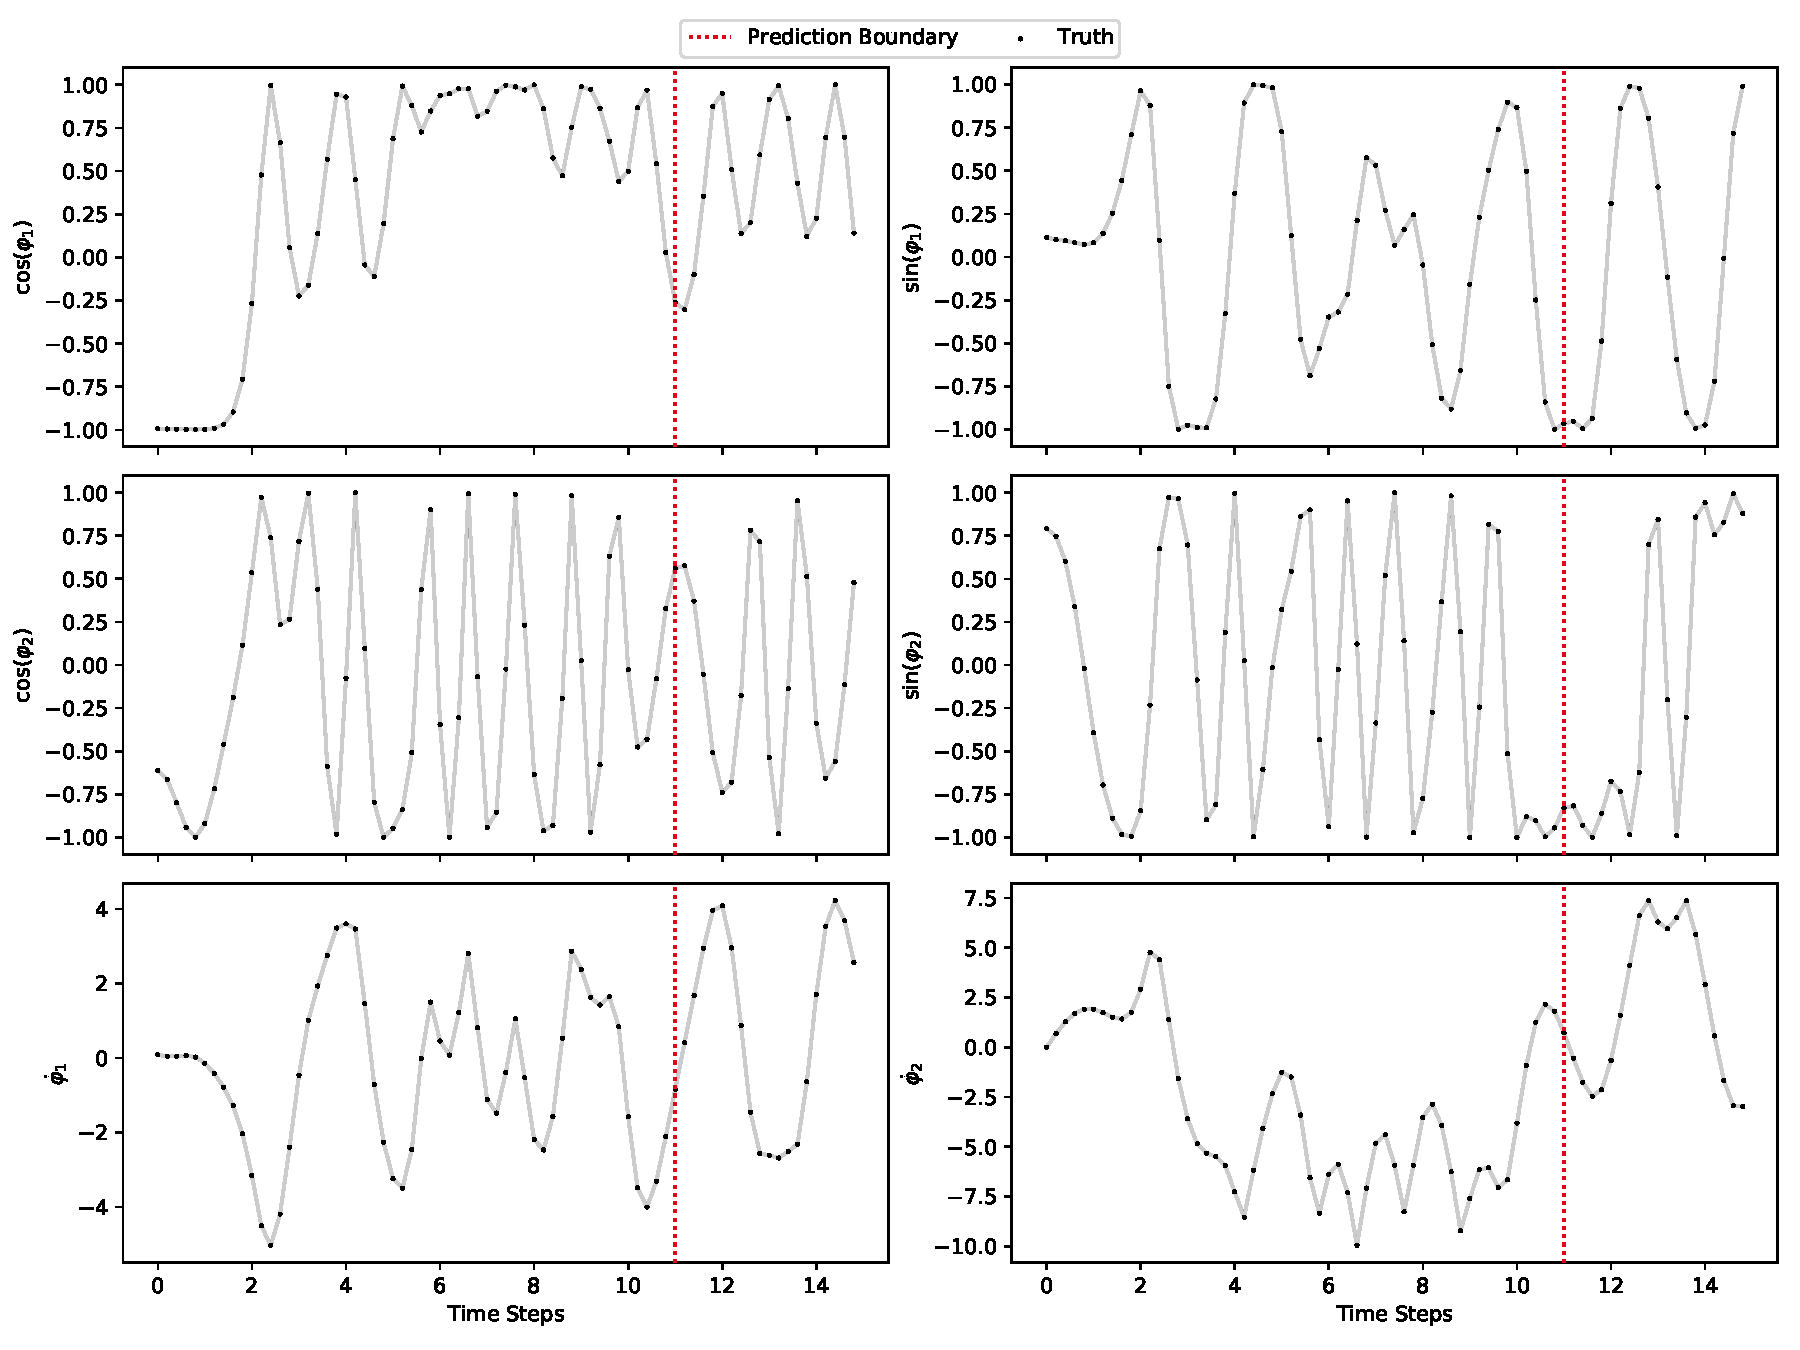
\includegraphics[width=\linewidth]{figures/experiments/environments/observations-acrobot-gym-N0.pdf}
				\caption{Plot of the raw data used for training the Gym double pendulum environment. The top row shows the cosine/sine of the displacement of the inner pendulum, the middle row shows the cosine/sine of the displacement of the outer pendulum and the bottom row shows the angular velocity of the inner and outer pendulum. The black dots represent the actual data points, all before the red prediction boundary are used for training, the rest for validation. The faint gray line emphasizes the connection between the data points and that they are actually generated from a dynamical system.}
				\label{fig:envDoublePendulumGym}
			\end{figure}
		% end
	% end

	\subsection{Experiment Setup}
		We will now introduce the experiment setup, initialization and similar stuff we used for each environment. For all experiments, we initialized the latent state dynamics matrix \( \mat{A} \) with an identity matrix, the initial state \( \vec{m}_0 \) with a one-vector and all covariance matrices \( \mat{R} \), \( \mat{R} \) and \( \mat{V}_0 \) with a small diagonal covariance of \( 10^{-5} \). We set the maximum number of \(\vec{g}\)-optimization iterations to \(1000\) for all environments. As described in~\autoref{sec:implementation}, we used a neural network for the observation function with \(\tanh\) activation functions (except for the output layer of course) and a single hidden layer with \(50\) neurons. The environment-specific parameters and the hidden layer sizes are given in~\autoref{tab:experimentSetup}.

		\todo{Update table once more results are here and we changed hyperparameters!}
		\begin{table}
			\centering
			\begin{tabular}{c|ccc}
				\textbf{Environment} & \textbf{Whitening?} & \textbf{Latent Dim.} & \textbf{Max. Iterations} \\ \hline
				      Pendulum       &         no          &        \(10\)        &         \(100\)          \\
				  Damped Pendulum    &         yes         &        \(10\)        &         \(200\)          \\
				    Gym Pendulum     &         no          &        \(10\)        &         \(500\)          \\
				    Gym Cartpole     &         yes         &        \(8\)         &         \(500\)          \\
				    Gym Acrobot      &         no          &        \(16\)        &         \(350\)
			\end{tabular}
			\caption{Overview over the different hyperparameter setting for the different environments.}
			\label{tab:experimentSetup}
		\end{table}

		For the proof-of-concept environment (the linear system), we used a slightly different setup as the environment is a lot simpler. We used a zero-layer neural network with no activation function, \ac{ie} a learnable matrix/linear transformation. We also fix the latent dimensionality to be \(2\) for the linear system as we only have two states.
	% end

	\subsection{Hyper-Experiments}
		Besides the performance on specific environments, we where interested in how hyperparameters like the latent dimensionality affect the performance of the system. In this section we will discuss and present our experiment setup for the "hyper-experiments". All hyperparameters that are not part of the experiment where set to the ones listed in~\autoref{tab:experimentSetup}.

		If not stated differently, we always ran the experiment with five different seeds\footnote{Namely, we used the seeds \(0\), \(11\), \(42\), \(1234\) and \(1997\) that where chosen on a random basis.} to average out initialization noise.

		\subsubsection{Influence of the Latent Dimensionality}
			\label{subsec:experimentLatentDim}

			As the latent dimensionality directly influences how well the Koopman matrix can approximate the infinite-dimensional operator, it is one of the most interesting hyperparameters we evaluated. Hence, we evaluated lots of different latent dimensionalities from \( k = 1 \) to \( k = 50 \) (for cartpole, we did \( k = 1, 2, \rangedots, 100 \)).
		% end
	% end
% end

\section{Results}
	\label{sec:results}

	\todo{Update all results with the latest results from the GPU!}

	In this section we will look at the results of the experiments described above. We organized the section into the different environments and will take a look at both the hyper-experiments first and then the individual results for optimized hyperparameters.

	For evaluating the performance of the model, we use different measures and metrics, both qualitative and quantitative. For a qualitative evaluation, we simply plot the produced data. These plots can get quite noisy as we will see, but they comprise all things we need for a qualitative assessment:
	\begin{itemize}
		\item The \emph{ground truth}, generated as described above with the adequate numerical integration of the equations of motion.
		\item The \emph{smoothed states} as they are produced from the E-step of the \algname algorithm, \ac{ie} \(\hat{\vec{s}}_{1:T}\).
		\item The \emph{rollout}, starting both from the learned initial value as well as from the last smoothed state. While the former visualizes the ability of the model to work completely "on its own", the latter shows how well the linear dynamics generalize beyond the training data.
		\item And of course the confidence (\ac{ie} the learned variance) around each trajectory.
	\end{itemize}
	For quantitative comparison, we focus on the \ac{nrmse} across all dimensions and time steps, computed as
	\begin{equation*}
		\mathit{NRMSE} = \frac{1}{k} \sum_{i = 1}^{k} \frac{1}{y_\mathrm{max} - y_\mathrm{min}} \sqrt{ \frac{1}{T} \sum_{t = 1}^{T} (y_{t, i} - \tilde{y}_{t, i})^2 }
	\end{equation*}
	where \( y_{t, i} \) is the true data and \( \tilde{y}_{t, i} \) is the corresponding data to evaluate at the \(t\)-th time step of the \(i\)-th dimension. We can compute four different error values: The error over the rollout from start to finish (\( t = 1, 2, \rangedots, T \)), over the training data only (\( t = 1, 2, \rangedots, T_\train \)), over the prediction only (\( t = T_\train, T_\train + 1, \rangedots, T \)) or over the smoothed trajectory (\ac{ie} the results from the E-step, \(  \hat{\vec{s}}_{1:T} \)). The latter primarily checks that our algorithm performs correct and that it is even capable of learning the dynamics and it should be near zero or at least below one for a decent parameter choice and model performance. On the other hand, the \ac{nrmse} over the complete rollout describes the generalization abilities. In conjunction with the rollout error over the training and prediction set, we can see where our error comes from. A low error over the training set is the least we should expect while at some environments a high error on the prediction is expected (we will later see when and why).

	Using the \ac{nrmse} instead of the plain \ac{rmse} allows us to compare model performance across the difference dimensions as we are scaling the error to a reasonable interval. For error values below \( 0.01 \), we say that the error is close to zero as it only deviates at most \(1\%\) from the true data. For \(<0.1\) we say it is a good fit, and for \(<0.2\) we say the approximation is decent. However, we have to take these numbers with care as they summarize a lot of data into a single scalar.

	All subsections (of non-proof-of-concept environments) are separated into two main parts: Looking at the hyper-experiment of the latent dimensionality and inspect how well the model performs with different latent dimensionalities. Then we will pick two or three of those latent dimensionalities and look at the qualitative plots of the runs (exemplary evaluation).

	Each exemplary evaluation also contains the ID of the run containing the data we used and the raw data of the runs is added to the GitHub repository along with the code. The documentation for how to generate the plots and so on is also there.

	\subsection{Proof-of-Concept: LGDS}
		For the \ac{lgds} environment, we did not run multiple latent dimensionalities as we already know how many states we have.~\autoref{fig:lgdsRollout} shows the rollout plot for \( k = 3 \) latent dimensions. As expected, the both the rollout and the smoothed states perfectly match the true data, even in the prediction time span.

		\begin{figure}
			\centering
			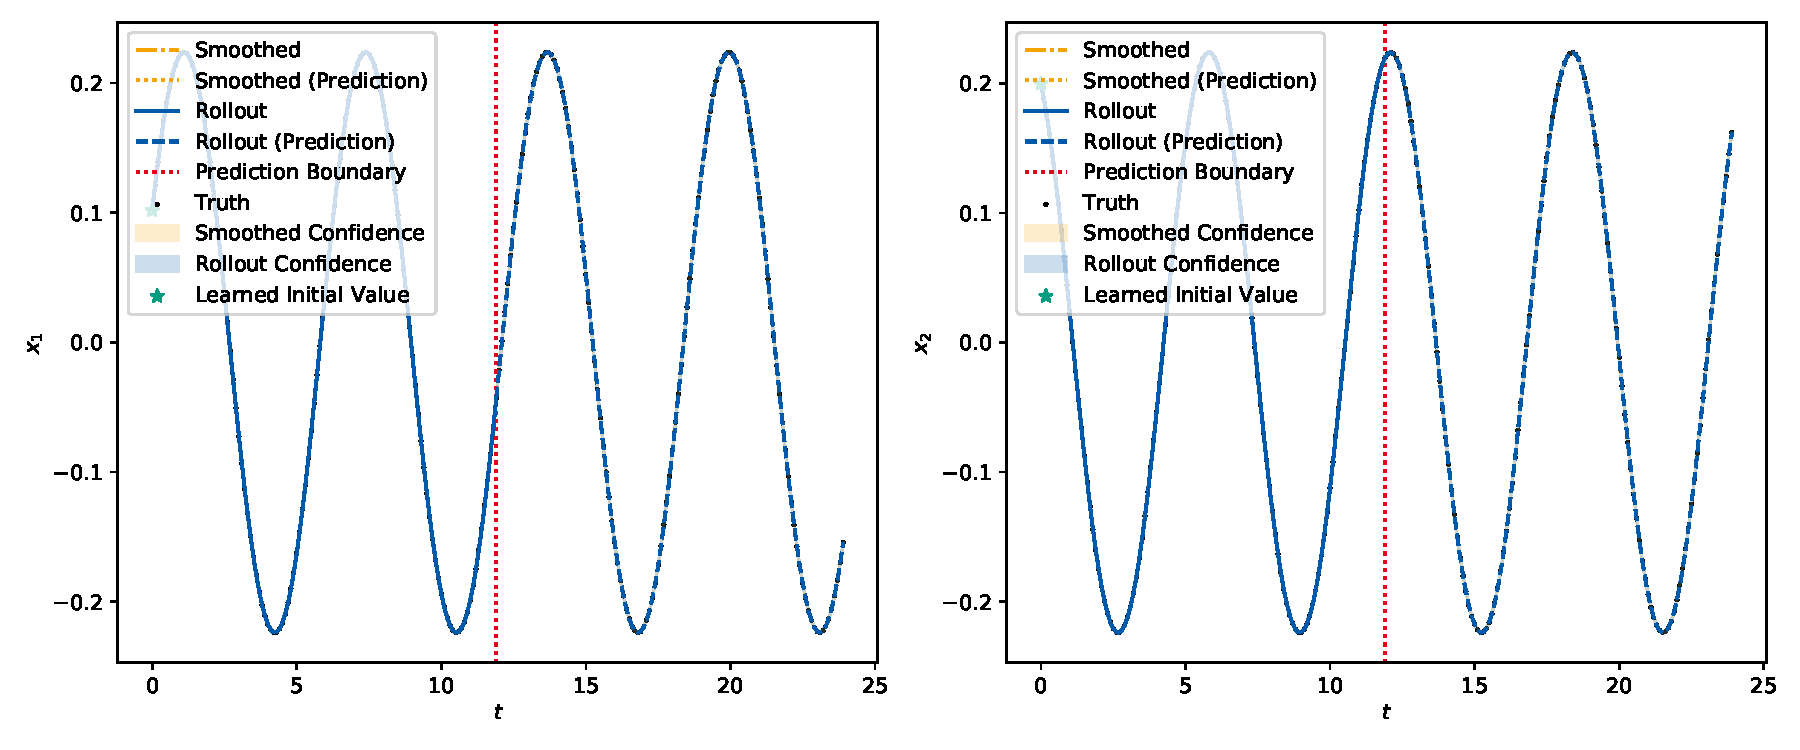
\includegraphics[width=\linewidth]{figures/results/lgds/rollout-observations-N0.pdf}
			\caption{The rollout plot in the observation space of the \ac{lgds} environment for \(k = 3\). The left plot shows the first dimension, the right plot the second dimension. The black dots represent the true data of which the model used everything till the red prediction boundary to train on. The blue line is the rollout, starting from the learned initial value (marked with a green star). The orange dash-dotted line is the smoothed data. The dotted orange line then is the rollout starting from the last smoothed state, forming the "smoothed prediction". The shaded regions show the confidence, \ac{ie} two times the standard deviation.}
			\label{fig:lgdsRollout}
		\end{figure}
	% end

	\subsection{Pendulum}
		\subsubsection{Influence of the Latent Dimensionality}
			For the pendulum experiment, we tested \(50\) latent dimensionalities from \( k = 1 \) to \( k = 50 \).

			We will start by having a first look at the \ac{nrmse} of the smoothed trajectory in~\autoref{fig:pendulumRmseSmoothed} to see how many latent dimensions we need the least to get a model that is even slightly capable of learning the pendulum dynamics. We see that the \ac{nrmse} shrinks to near zero (less than \( 0.01 \)). Even for \( k = 1 \), the error is only approx. \( 0.18 \).

			Looking at the \ac{nrmse} of the complete rollout in~\autoref{fig:pendulumRmseComplete}, we see that the error is quite noisy due to initialization. Nevertheless, the error shrinks until \( k \geq 10 \) and then stabilizes around an error of approx. \(0.15\). Comparing the complete rollout error with the training and prediction \ac{nrmse} in~\autoref{fig:pendulumRmseTrain} and~\autoref{fig:pendulumRmsePred}, respectively, we see that the training error falls until \( k \geq 10 \) and then stabilizes around \(0.08\). For the prediction error, we see a similar connection to \( k \geq 10 \), but the error does not shrink as much and always is around \(0.20\).

			\begin{figure}
				\centering
				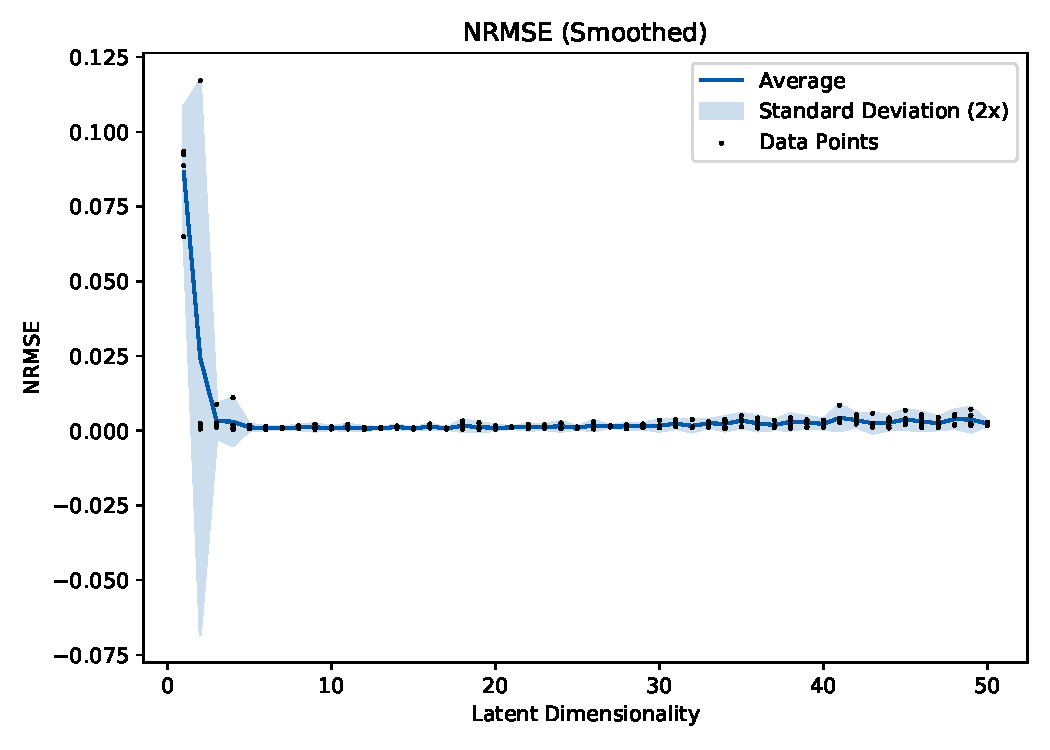
\includegraphics[width=0.7\linewidth]{figures/results/pendulum-damped/latent-dim/comparison-rmse-smoothed-normalized-mean-vs-latent-dim.pdf}
				\caption{The \ac{nrmse} of the smoothed trajectory on the training data of the damped pendulum environment.}
				\label{fig:pendulumRmseSmoothed}
			\end{figure}

			\begin{figure}
				\centering
				\begin{subfigure}{0.7\linewidth}
					\centering
					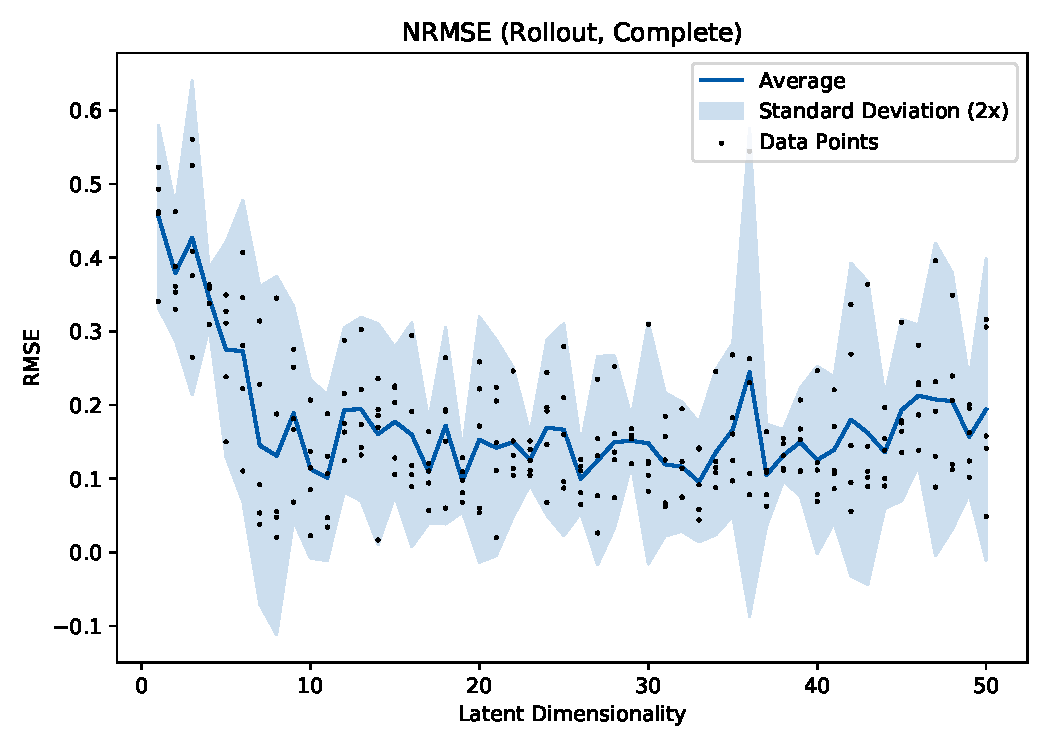
\includegraphics[width=\linewidth]{figures/results/pendulum/latent-dim/comparison-rmse-rollout-normalized-mean-vs-latent-dim.pdf}
					\caption{Error of the complete rollout on the pendulum environment.}
					\label{fig:pendulumRmseComplete}
				\end{subfigure} \\
				\begin{subfigure}{0.5\linewidth}
					\centering
					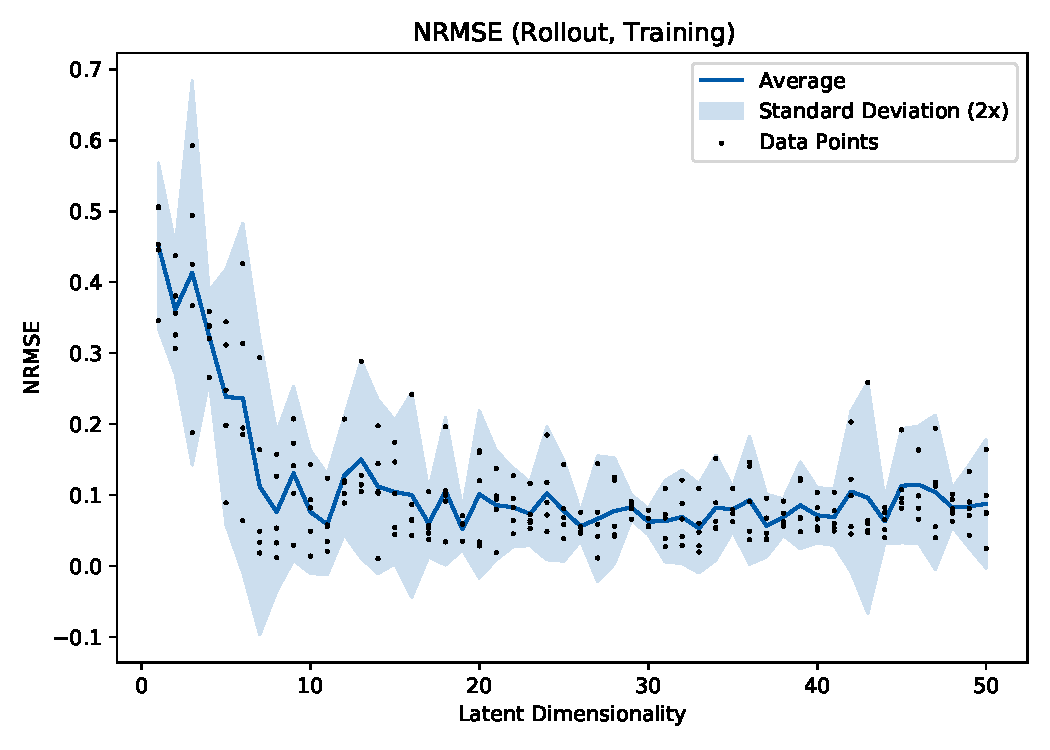
\includegraphics[width=\linewidth]{figures/results/pendulum/latent-dim/comparison-rmse-rollout-train-normalized-mean-vs-latent-dim.pdf}
					\caption{Error of the rollout on the training data only on the pendulum environment.}
					\label{fig:pendulumRmseTrain}
				\end{subfigure}%
				~
				\begin{subfigure}{0.5\linewidth}
					\centering
					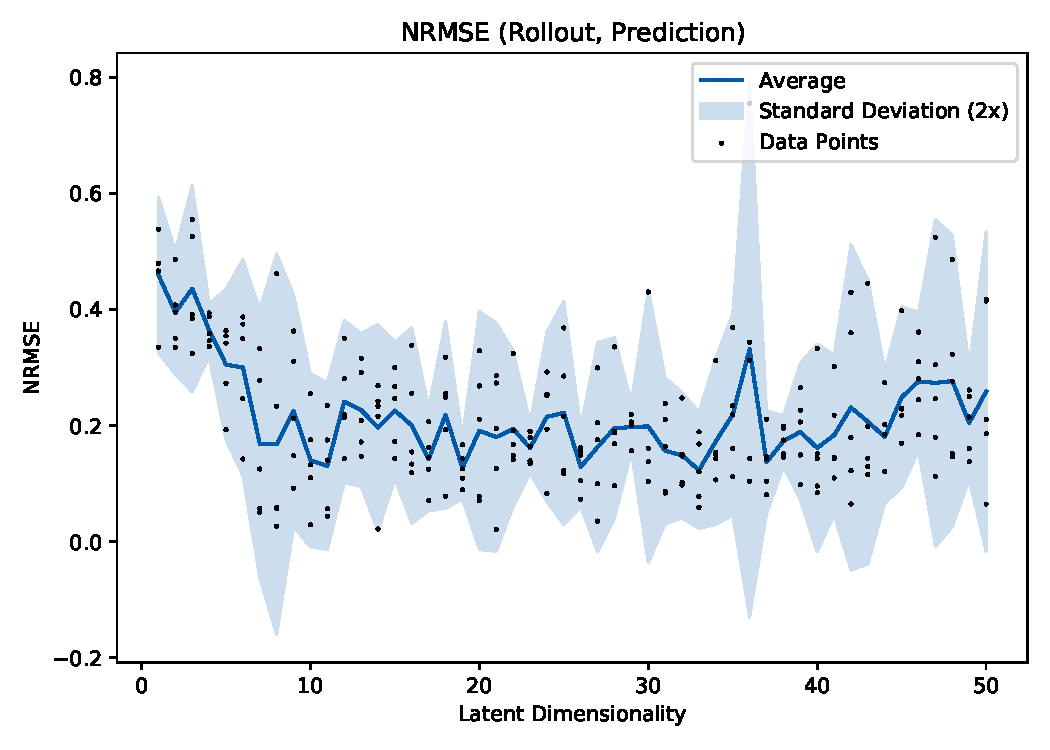
\includegraphics[width=\linewidth]{figures/results/pendulum/latent-dim/comparison-rmse-rollout-prediction-normalized-mean-vs-latent-dim.pdf}
					\caption{Error of the rollout on the prediction only on the pendulum environment.}
					\label{fig:pendulumRmsePred}
				\end{subfigure}
				\caption{Plot of the errors of the pendulum environment for different latent dimensions. The black dots show the measured data, the blue line the average of the data points at a specific time step. The blue shaded region shows two times the standard deviation.}
				\label{fig:pendulumRmse}
			\end{figure}
		% end

		\subsubsection{Exemplary Evaluation: 2-Dimensional Latent}
			We will now look at an exemplary run for the latent dimensionality \( k = 2 \) (run \texttt{100}). According to the errors, the rollout error should be quite high. On the other hand, the smoothed trajectory should nearly match the true data.~\autoref{fig:pendulumRolloutL02} shows that the rollout and also the rollout of the smoothed trajectory are far off with low confidence, but the true data is in the confidence region. However, the smoothed trajectory follows the true data really good.

			\begin{figure}
				\centering
				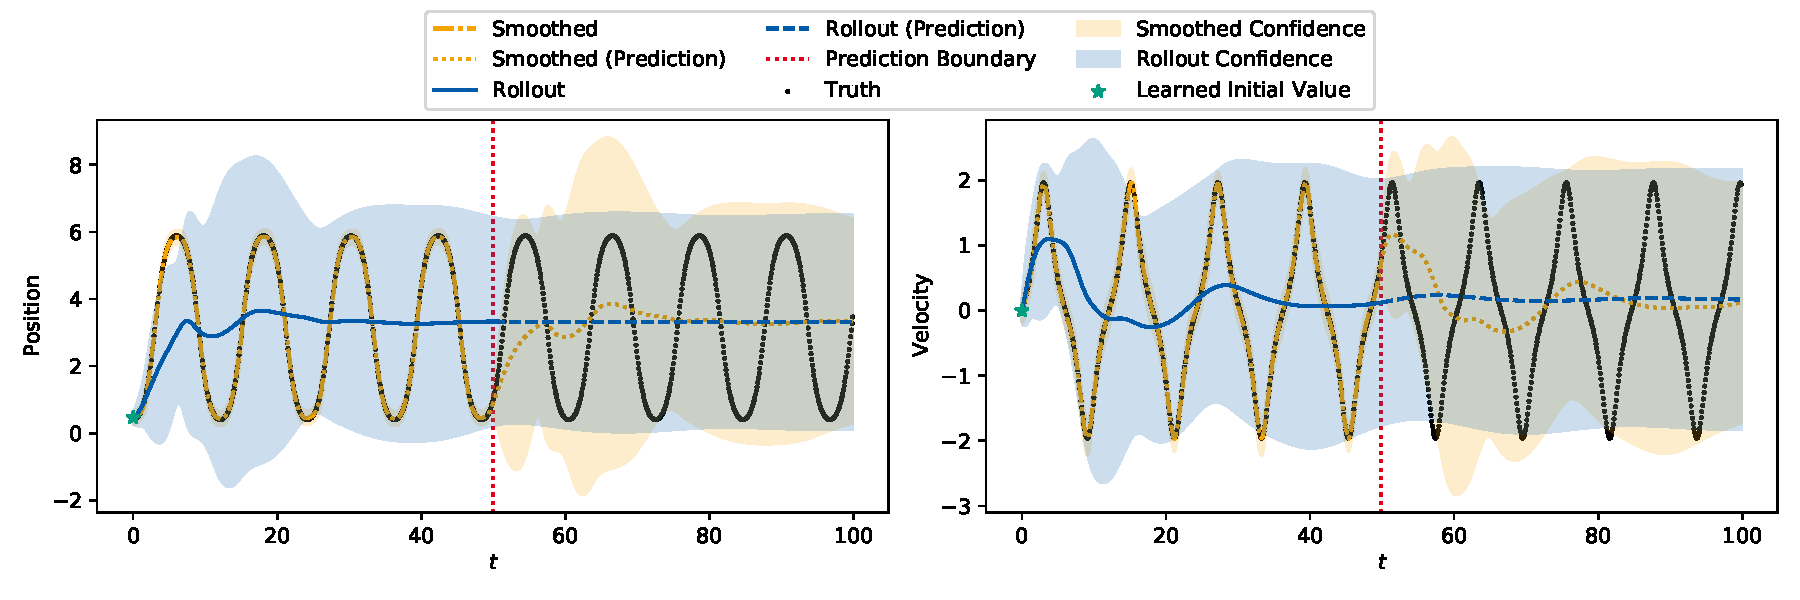
\includegraphics[width=\linewidth]{figures/results/pendulum/run-latent-dim-02/rollout-observations-N0.pdf}
				\caption{The rollout plot in the observation space of the pendulum environment for \(k = 2\). The left plot shows the displacement and the right plot the angular velocity. The black dots represent the true data of which the model used everything till the red prediction boundary to train on. The blue line is the rollout, starting from the learned initial value (marked with a green star). The orange dash-dotted line is the smoothed data. The dotted orange line then is the rollout starting from the last smoothed state, forming the "smoothed prediction". The shaded regions show the confidence, \ac{ie} two times the standard deviation.}
				\label{fig:pendulumRolloutL02}
			\end{figure}
		% end

		\subsubsection{Exemplary Evaluation: 4-Dimensional Latent}
			We will now look at an exemplary run for the latent dimensionality \( k = 4 \) (run \texttt{53}). This run is especially interesting for comparison with~\cite{mortonDeepVariationalKoopman2019a} which we will do in~\autoref{c:discussion}.~\autoref{fig:pendulumRolloutL04} shows the rollout of the model with four latent dimensions. We see that the smoothed trajectory equals the true data as expected, while the rollout captures the dynamics of the system really roughly and the true data lies withing the region of confidence of the rollout.

			\begin{figure}
				\centering
				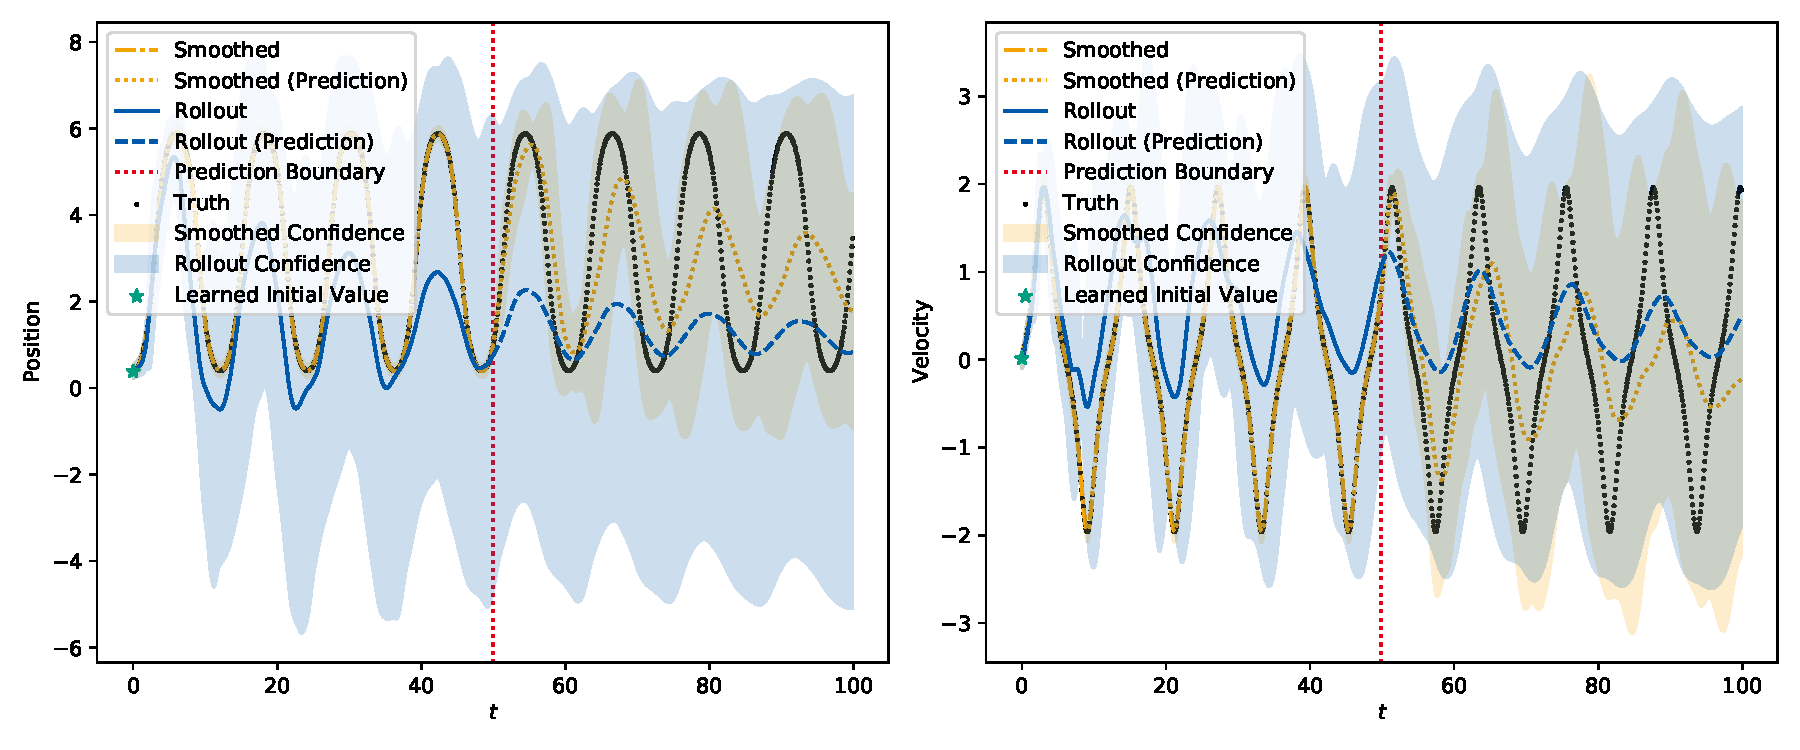
\includegraphics[width=\linewidth]{figures/results/pendulum/run-latent-dim-04/rollout-observations-N0.pdf}
				\caption{The rollout plot in the observation space of the pendulum environment for \(k = 4\). The left plot shows the displacement and the right plot the angular velocity. The black dots represent the true data of which the model used everything till the red prediction boundary to train on. The blue line is the rollout, starting from the learned initial value (marked with a green star). The orange dash-dotted line is the smoothed data. The dotted orange line then is the rollout starting from the last smoothed state, forming the "smoothed prediction". The shaded regions show the confidence, \ac{ie} two times the standard deviation.}
				\label{fig:pendulumRolloutL04}
			\end{figure}
		% end

		\subsubsection{Exemplary Evaluation: 10-Dimensional Latent}
			\label{subsubsec:pendulumL10}

			We will now look at an exemplary run for the latent dimensionality \( k = 10 \) (run \texttt{10}) as we postulated from the \ac{nrmse} data that this is the boundary of diminishing returns, \ac{ie} it does not get much better with higher latent dimensionalities.~\autoref{fig:pendulumRolloutL10} shows the rollout of the model, where the dynamics of the system are captured really good with high confidence. Also the prediction is really good, so that it is hard to distinguish between true data, smoothed prediction and rollout.

			\begin{figure}
				\centering
				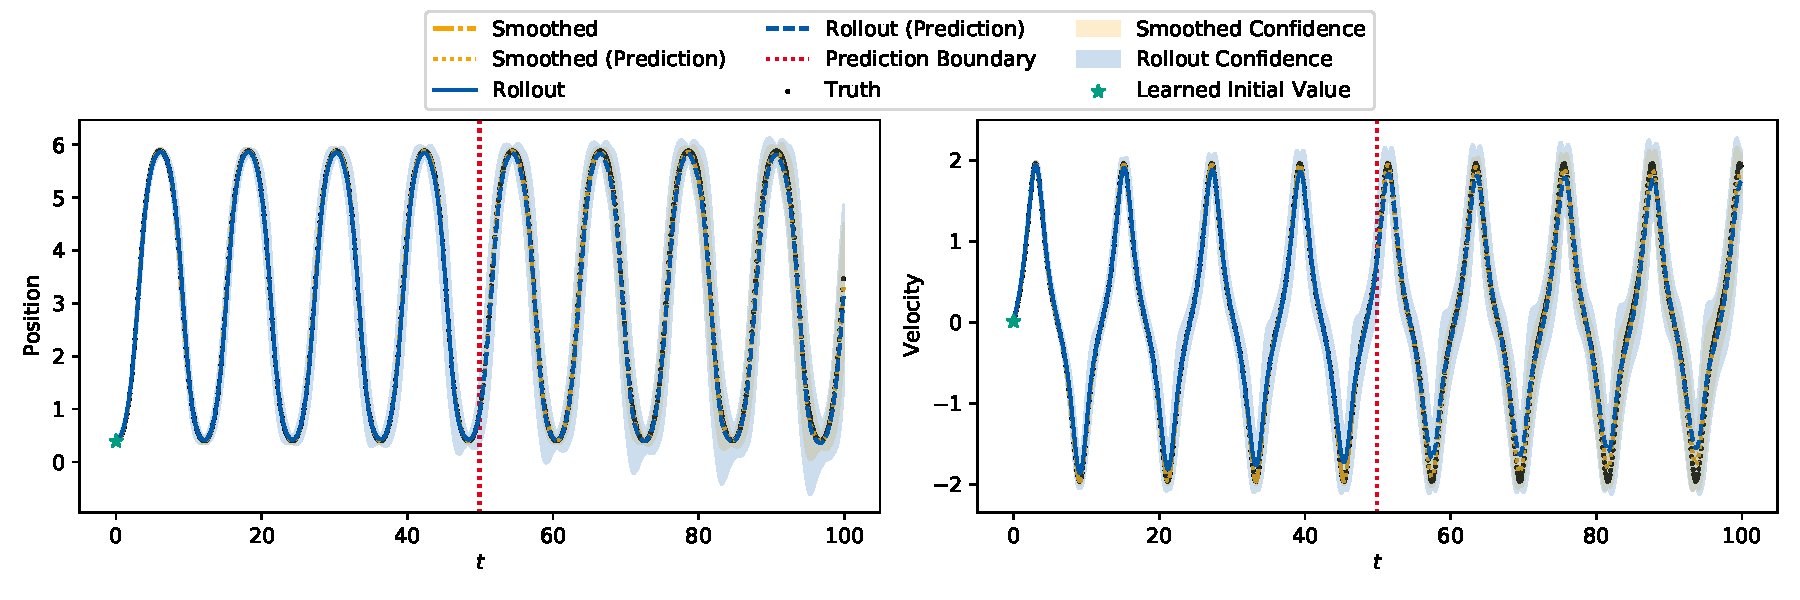
\includegraphics[width=\linewidth]{figures/results/pendulum/run-latent-dim-10/rollout-observations-N0.pdf}
				\caption{The rollout plot in the observation space of the pendulum environment for \(k = 10\). The left plot shows the displacement and the right plot the angular velocity. The black dots represent the true data of which the model used everything till the red prediction boundary to train on. The blue line is the rollout, starting from the learned initial value (marked with a green star). The orange dash-dotted line is the smoothed data. The dotted orange line then is the rollout starting from the last smoothed state, forming the "smoothed prediction". The shaded regions show the confidence, \ac{ie} two times the standard deviation.}
				\label{fig:pendulumRolloutL10}
			\end{figure}
		% end

		\subsubsection{Exemplary Evaluation: 14-Dimensional Latent}
			\label{subsubsec:pendulumL14}

			We will now look at an exemplary run for the latent dimensionality \( k = 14 \) (run \texttt{210}) for which we got the smallest overall \ac{nrmse}.~\autoref{fig:pendulumRolloutL14} shows the rollout of the model. In comparison to the 10-dimensional latent, nothing has changed, fulfilling the expectation of diminishing returns with high latent dimensionality.

			\begin{figure}
				\centering
				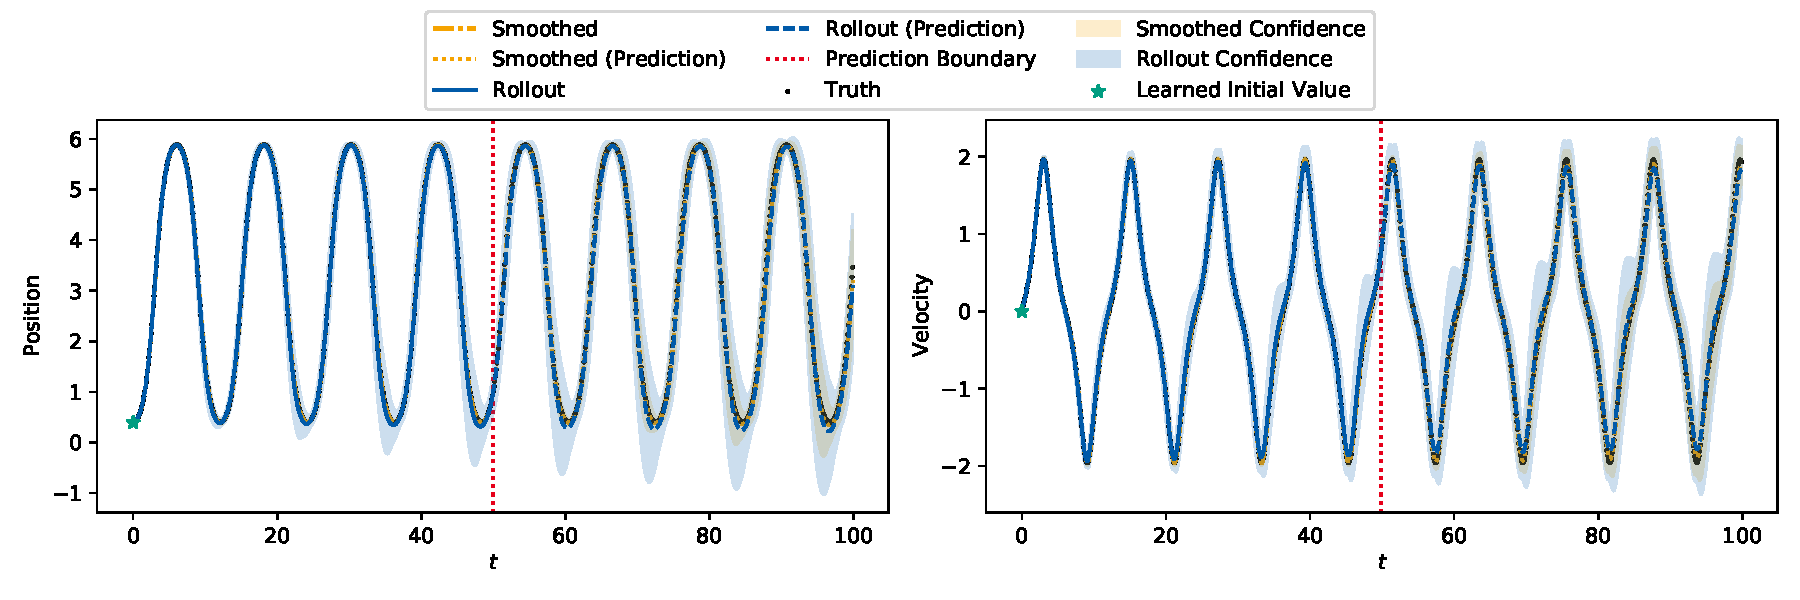
\includegraphics[width=\linewidth]{figures/results/pendulum/run-latent-dim-14/rollout-observations-N0.pdf}
				\caption{The rollout plot in the observation space of the pendulum environment for \(k = 14\). The left plot shows the displacement and the right plot the angular velocity. The black dots represent the true data of which the model used everything till the red prediction boundary to train on. The blue line is the rollout, starting from the learned initial value (marked with a green star). The orange dash-dotted line is the smoothed data. The dotted orange line then is the rollout starting from the last smoothed state, forming the "smoothed prediction". The shaded regions show the confidence, \ac{ie} two times the standard deviation.}
				\label{fig:pendulumRolloutL14}
			\end{figure}
		% end
	% end

	\subsection{Damped Pendulum}
		\subsubsection{Influence of the Latent Dimensionality}
			For the damped pendulum experiment, we tested \(50\) latent dimensionalities from \( k = 1 \) to \( k = 50 \).

			We will start by having a first look at the \ac{nrmse} of the smoothed trajectory in~\autoref{fig:pendulumDampedRmseSmoothed} to see how many latent dimensions we need the least to get a model that is even slightly capable of learning the damped pendulum dynamics. We see that the \ac{nrmse} shrinks to near zero (less than \( 0.01 \)) for latent dimensionalities of \( k \geq 2 \). Even for \( k = 1 \), the error is only approx. \( 0.09 \).

			Looking at the \ac{nrmse} of the complete rollout in~\autoref{fig:pendulumDampedRmseComplete}, we see that there is a point of diminishing returns in terms of the latent dimensionality for \( k \geq 10 \), where we get decent errors (around \( 0.05 \)) for all latent dimensionalities. Looking at the parts the complete \ac{nrmse} is composed of, the training and prediction error in~\autoref{fig:pendulumDampedRmseTrain} and~\autoref{fig:pendulumDampedRmsePred}, respectively, we see that the latent dimensionality affects both parts, the training and prediction error. However, the prediction error in generally smaller, which is mostly caused by the value of the state and hence the rollout being smaller.

			\begin{figure}
				\centering
				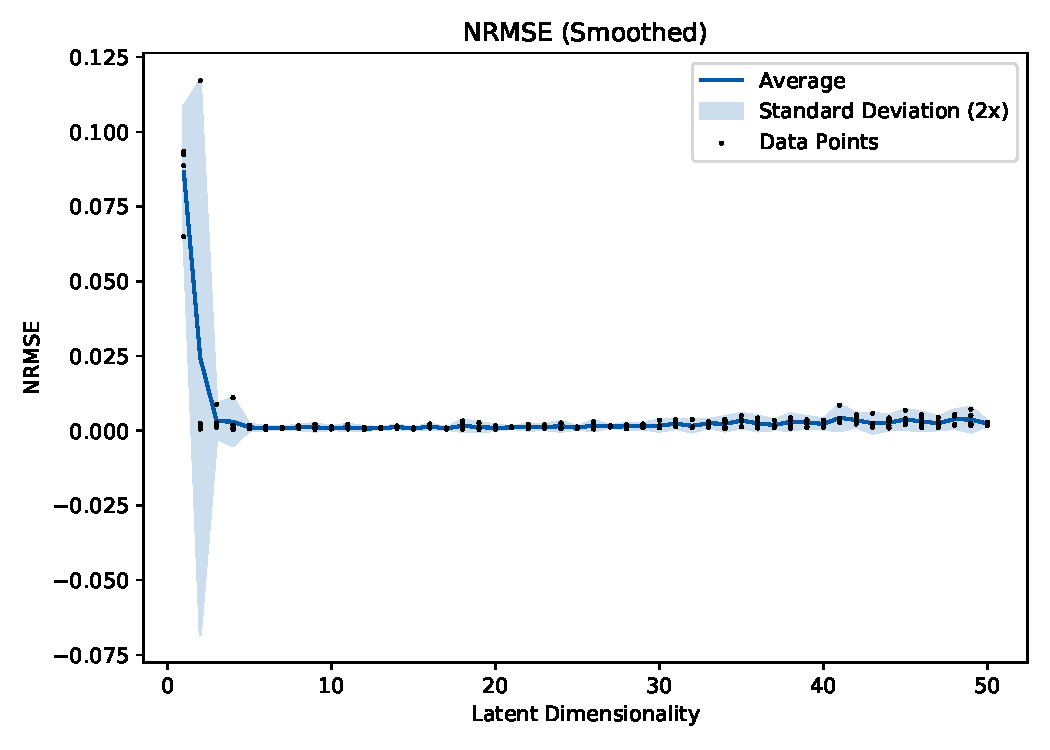
\includegraphics[width=0.7\linewidth]{figures/results/pendulum-damped/latent-dim/comparison-rmse-smoothed-normalized-mean-vs-latent-dim.pdf}
				\caption{The \ac{nrmse} of the smoothed trajectory on the training data of the damped pendulum environment.}
				\label{fig:pendulumDampedRmseSmoothed}
			\end{figure}

			\begin{figure}
				\centering
				\begin{subfigure}{0.7\linewidth}
					\centering
					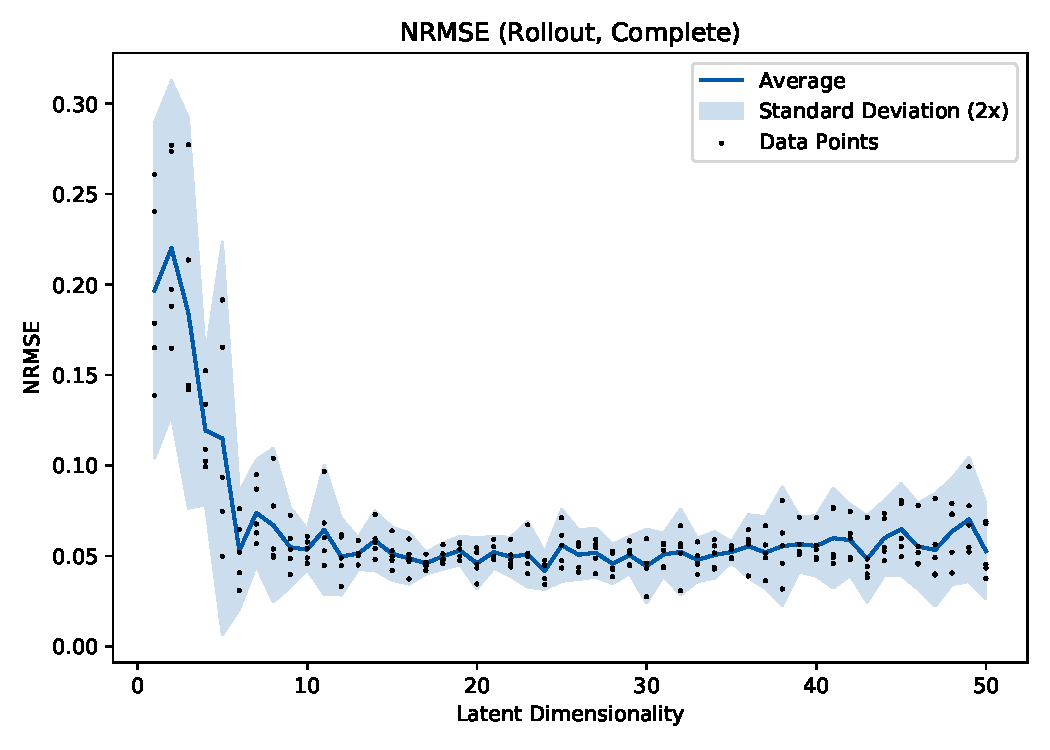
\includegraphics[width=\linewidth]{figures/results/pendulum-damped/latent-dim/comparison-rmse-rollout-normalized-mean-vs-latent-dim.pdf}
					\caption{Error of the complete rollout on the damped pendulum environment.}
					\label{fig:pendulumDampedRmseComplete}
				\end{subfigure} \\
				\begin{subfigure}{0.5\linewidth}
					\centering
					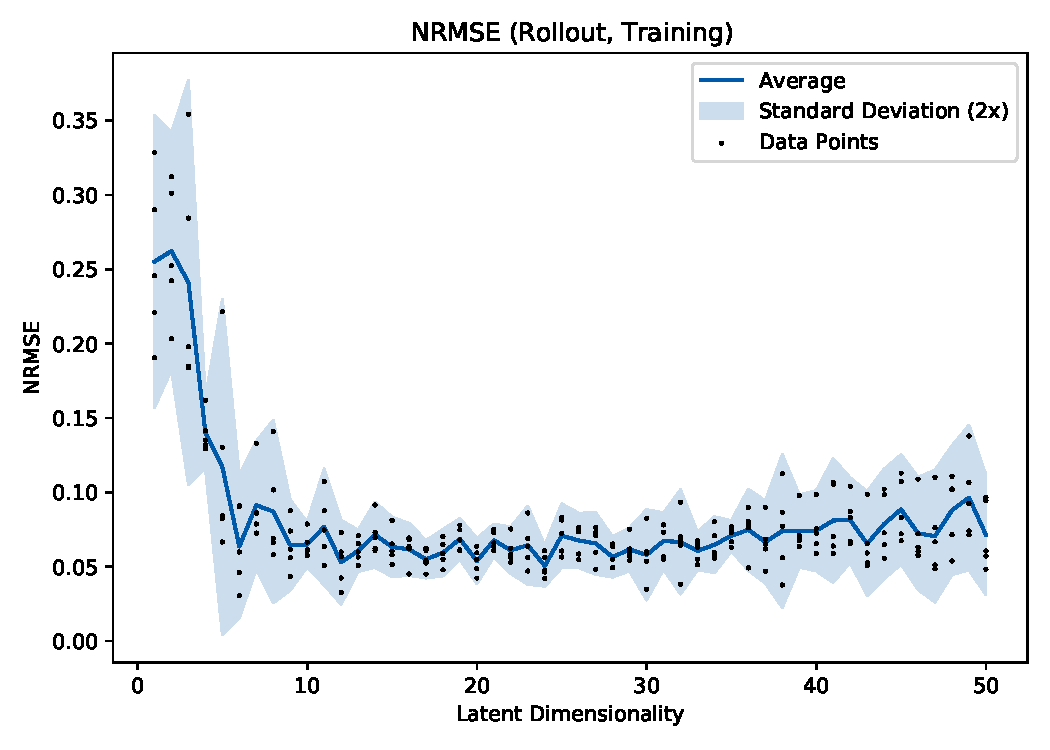
\includegraphics[width=\linewidth]{figures/results/pendulum-damped/latent-dim/comparison-rmse-rollout-train-normalized-mean-vs-latent-dim.pdf}
					\caption{Error of the rollout on the training data only on the damped pendulum environment.}
					\label{fig:pendulumDampedRmseTrain}
				\end{subfigure}%
				~
				\begin{subfigure}{0.5\linewidth}
					\centering
					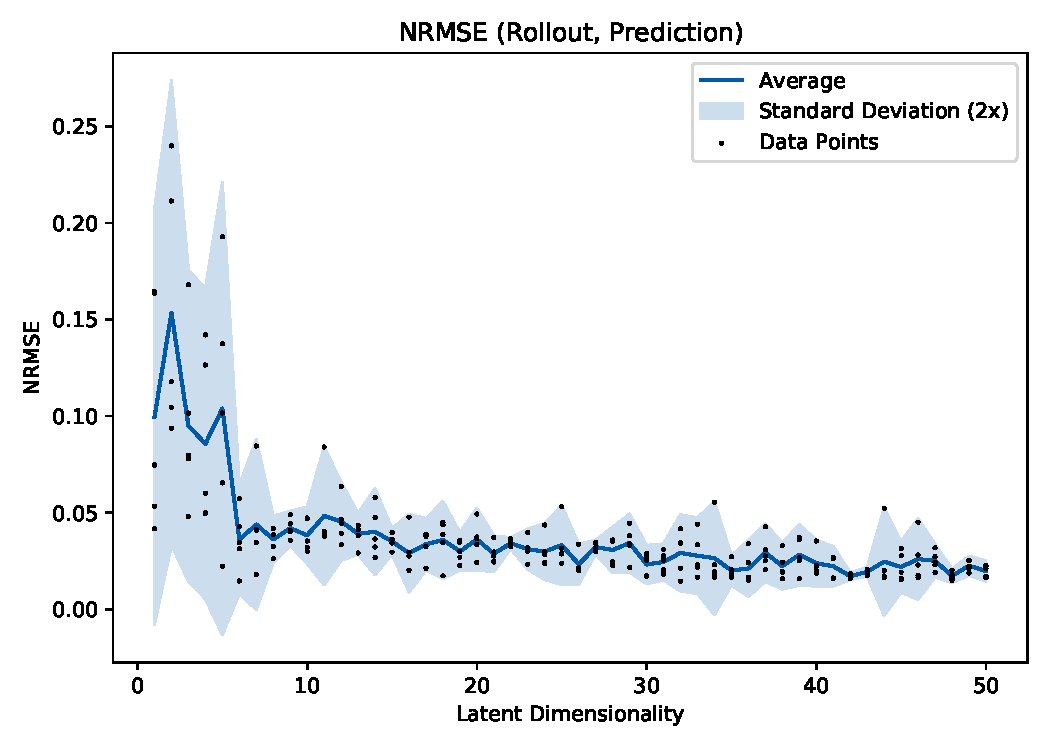
\includegraphics[width=\linewidth]{figures/results/pendulum-damped/latent-dim/comparison-rmse-rollout-prediction-normalized-mean-vs-latent-dim.pdf}
					\caption{Error of the rollout on the prediction only on the damped pendulum environment.}
					\label{fig:pendulumDampedRmsePred}
				\end{subfigure}
				\caption{Plot of the errors of the damped pendulum environment for different latent dimensions. The black dots show the measured data, the blue line the average of the data points at a specific time step. The blue shaded region shows two times the standard deviation.}
				\label{fig:pendulumDampedRmse}
			\end{figure}
		% end

		\subsubsection{Exemplary Evaluation: 2-Dimensional Latent}
			We will now look at an exemplary run for the latent dimensionality \( k = 2 \) (run \texttt{2}). According to the errors, the rollout error should be quite high, but the smoothed trajectory should follow the true data really good.~\autoref{fig:pendulumDampedRolloutL02} shows that most trajectories are far off the true trajectory with low confidence, while the smoothed trajectory nearly perfectly matches the true data.

			\begin{figure}
				\centering
				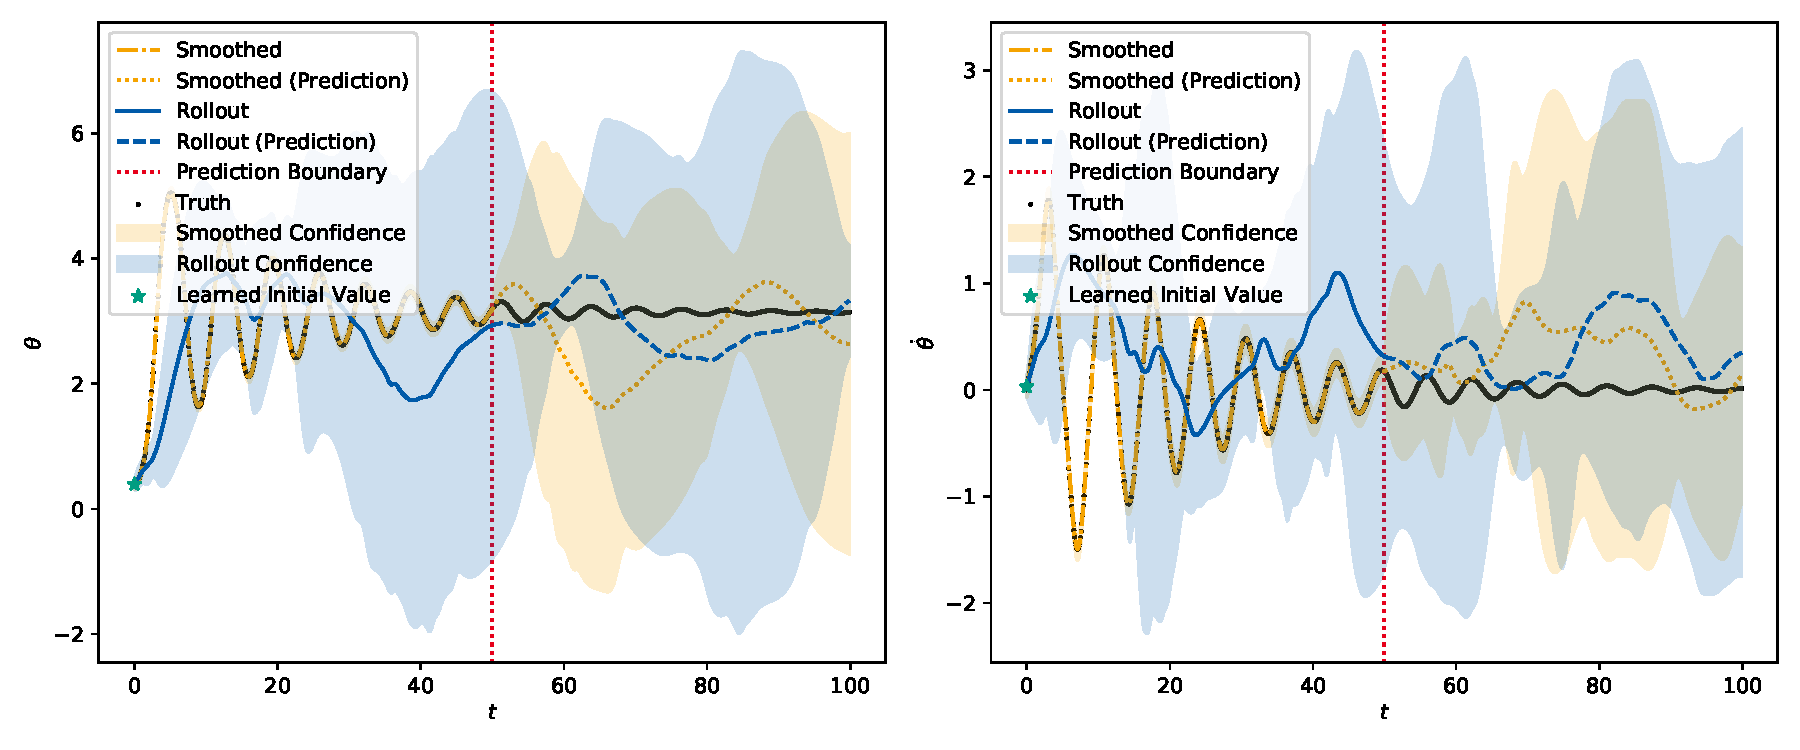
\includegraphics[width=\linewidth]{figures/results/pendulum-damped/run-latent-dim-02/rollout-observations-N0.pdf}
				\caption{The rollout plot in the observation space of the damped pendulum environment for \(k = 2\). The left plot shows the displacement and the right plot the angular velocity. The black dots represent the true data of which the model used everything till the red prediction boundary to train on. The blue line is the rollout, starting from the learned initial value (marked with a green star). The orange dash-dotted line is the smoothed data. The dotted orange line then is the rollout starting from the last smoothed state, forming the "smoothed prediction". The shaded regions show the confidence, \ac{ie} two times the standard deviation.}
				\label{fig:pendulumDampedRolloutL02}
			\end{figure}
		% end

		\subsubsection{Exemplary Evaluation: 10-Dimensional Latent}
			\label{subsubsec:pendulumDampedL10}

			We will now look at an exemplary run for the latent dimensionality \( k = 10 \) (run \texttt{110}). We chose this latent dimensionality as it is the boundary of diminishing returns in terms of the \ac{nrmse}, \ac{ie} it does not get much better from now on.~\autoref{fig:pendulumDampedRolloutL10} shows the rollout of the model. In comparison to the four-dimensional latent, the behavior of the system is captured pretty good, with a decent confidence. Also the prediction is at nearly the same amplitude as the real data. But the rollout gets phase-shifted in comparison to the true data further in the rollout horizon.

			\begin{figure}
				\centering
				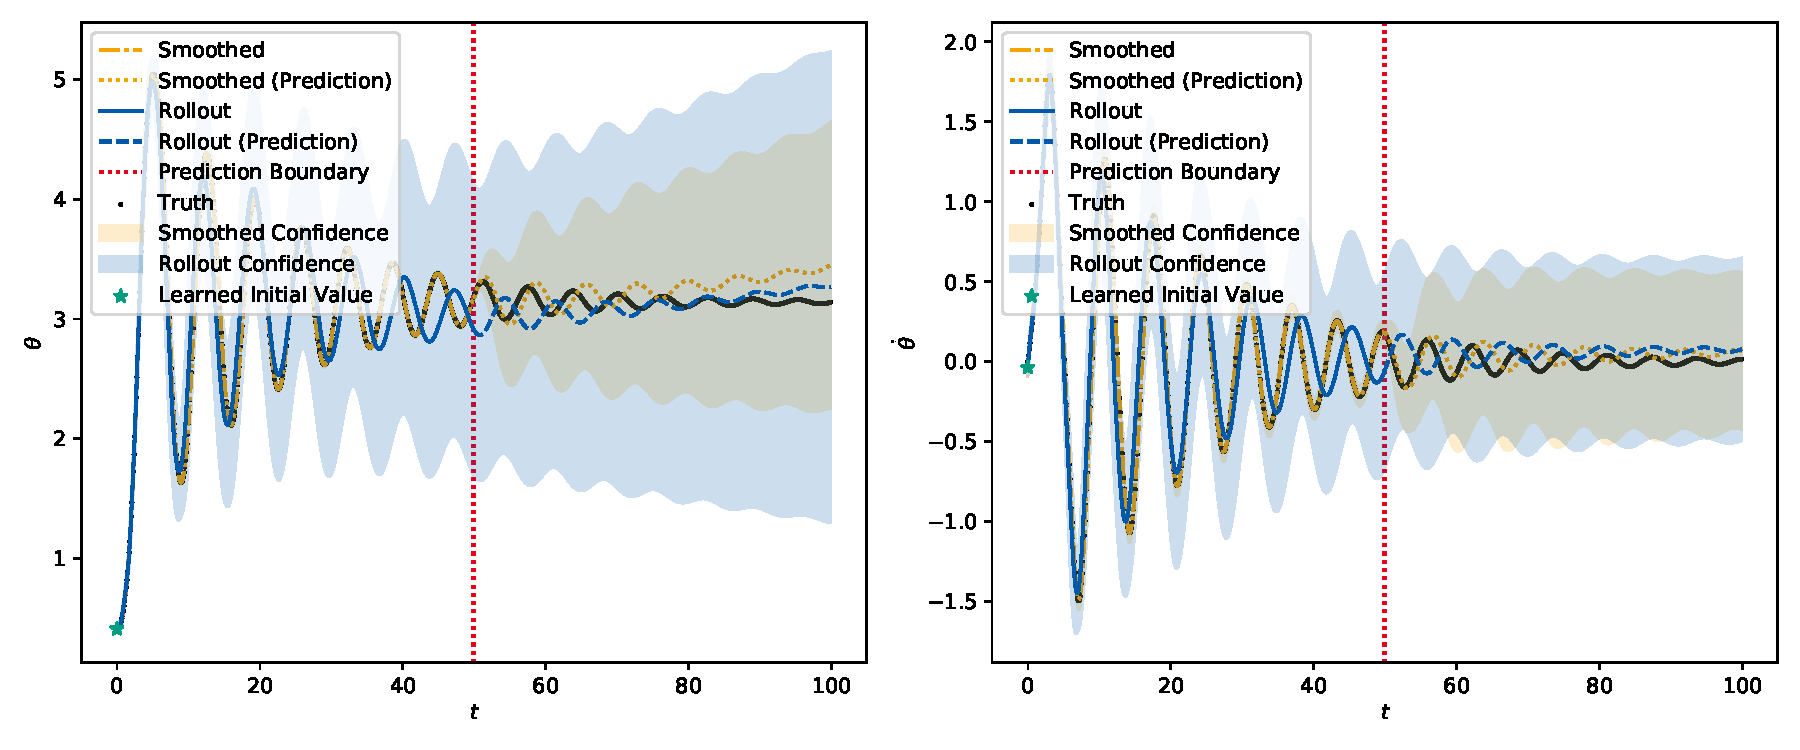
\includegraphics[width=\linewidth]{figures/results/pendulum-damped/run-latent-dim-10/rollout-observations-N0.pdf}
				\caption{The rollout plot in the observation space of the damped pendulum environment for \(k = 10\). The left plot shows the displacement and the right plot the angular velocity. The black dots represent the true data of which the model used everything till the red prediction boundary to train on. The blue line is the rollout, starting from the learned initial value (marked with a green star). The orange dash-dotted line is the smoothed data. The dotted orange line then is the rollout starting from the last smoothed state, forming the "smoothed prediction". The shaded regions show the confidence, \ac{ie} two times the standard deviation.}
				\label{fig:pendulumDampedRolloutL10}
			\end{figure}
		% end

		\subsubsection{Exemplary Evaluation: 24-Dimensional Latent}
			We will now look at an exemplary run for the latent dimensionality \( k = 30 \) (run \texttt{130}) for which we got the smallest overall \ac{nrmse}.~\autoref{fig:pendulumDampedRolloutL30} shows the rollout of the model. In comparison to the ten-dimensional latent, the model is a less confident but the rollout is nearly the same as the rollout of the ten-dimensional latent.

			\begin{figure}
				\centering
				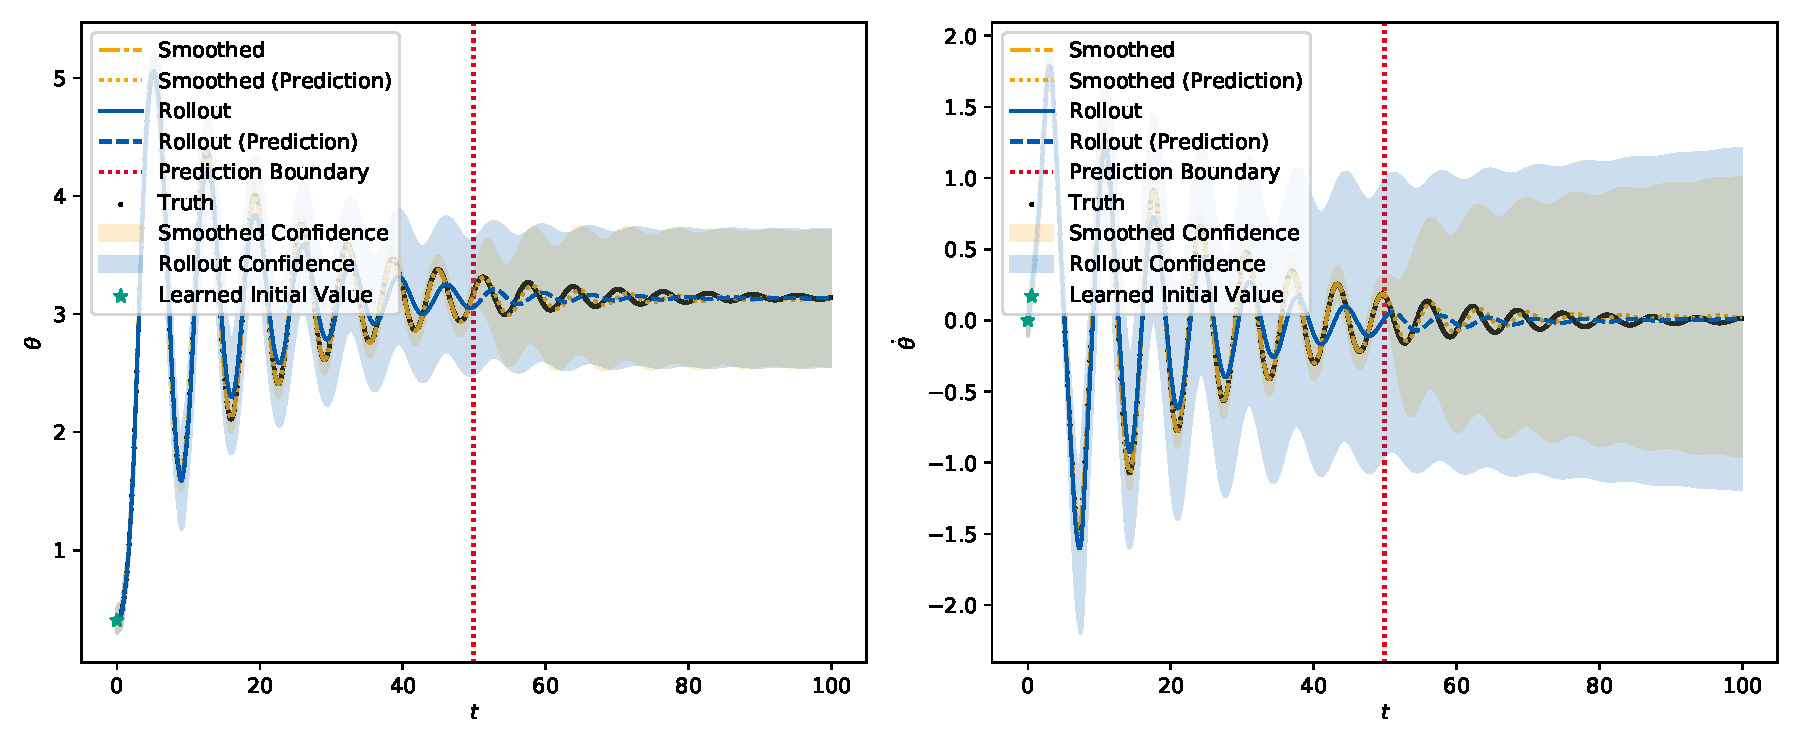
\includegraphics[width=\linewidth]{figures/results/pendulum-damped/run-latent-dim-30/rollout-observations-N0.pdf}
				\caption{The rollout plot in the observation space of the damped pendulum environment for \(k = 30\). The left plot shows the displacement and the right plot the angular velocity. The black dots represent the true data of which the model used everything till the red prediction boundary to train on. The blue line is the rollout, starting from the learned initial value (marked with a green star). The orange dash-dotted line is the smoothed data. The dotted orange line then is the rollout starting from the last smoothed state, forming the "smoothed prediction". The shaded regions show the confidence, \ac{ie} two times the standard deviation.}
				\label{fig:pendulumDampedRolloutL30}
			\end{figure}
		% end
	% end

	\subsection{Gym Pendulum}
		\todo{Update this section once more seeds have been tried! Numerical instabilities...}
		\todo{Include exemplary evaluations once data is here!}

		\subsubsection{Influence of the Latent Dimensionality}
			% This environment crashed nearly every time, so we do not have usable results yet :/

			\todo{Results: Gym Pendulum, Latent Dim.}
		% end
	% end

	\subsection{Gym Cartpole}
		\subsubsection{Influence of the Latent Dimensionality}
			For the cartpole experiment, we tested \(100\) latent dimensionalities from \( k = 1 \) to \( k = 100 \). Towards the end of this interval, the data points we where able to collect shrink (sometimes even to zero), as the algorithm increasingly numerically brittle with higher latent dimensionality (see also~\autoref{sec:implementation} for comments on the numerical stability).

			We will start by having a first look at the \ac{nrmse} of the smoothed trajectory in~\autoref{fig:cartpoleRmseSmoothed} to see how many latent dimensions we need the least to get a model that is even slightly capable of learning the cartpole dynamics. We see that the \ac{nrmse} shrinks to near zero for latent dimensionalities of \( k \geq 2 \). Hence, we need at least \(2\) latent dimensions to learn the dynamics.

			Looking at the \ac{nrmse} of the complete rollout in~\autoref{fig:cartpoleRmseComplete}, we see that the latent dimensionality does not really have an effect on how well we learn the dynamics. However, a look at the training and prediction \ac{nrmse} plots in~\autoref{fig:cartpoleRmseTrain} and~\autoref{fig:cartpoleRmsePred}, respectively, shows that the most errors is primarily caused by the prediction. Looking just at the training error, we see that we need at least \( k \geq 10 \) to get a nearly perfect error on the training data (below \(0.01\). As the data is quite noisy due to initialization errors, we might reach this boundary before, but starting from \(k \geq 10\) latent dimensions, most of the data points lie on the zero-line, so it is fair to say that the other runs where "just unlucky" in the initialization. Looking at the prediction plot, however, we see total randomness in the \ac{nrmse} with the average \ac{nrmse} across all latents being quite high (approx. \(0.44\)). Hence, we can safely say that our algorithm does not generalize well on the cartpole environment (we will look at potential reasons for this in~\autoref{c:discussion}).

			\begin{figure}
				\centering
				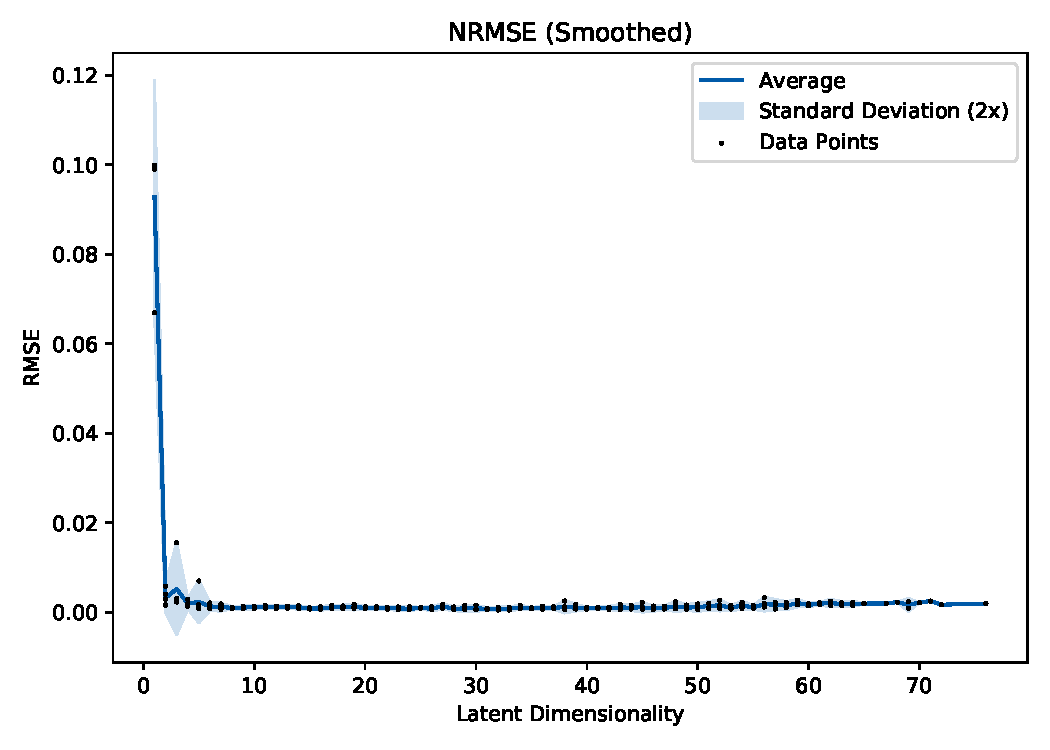
\includegraphics[width=0.7\linewidth]{figures/results/cartpole-gym/latent-dim/comparison-rmse-smoothed-normalized-mean-vs-latent-dim.pdf}
				\caption{The \ac{nrmse} of the smoothed trajectory on the training data of the cartpole environment.}
				\label{fig:cartpoleRmseSmoothed}
			\end{figure}

			\begin{figure}
				\centering
				\begin{subfigure}{0.7\linewidth}
					\centering
					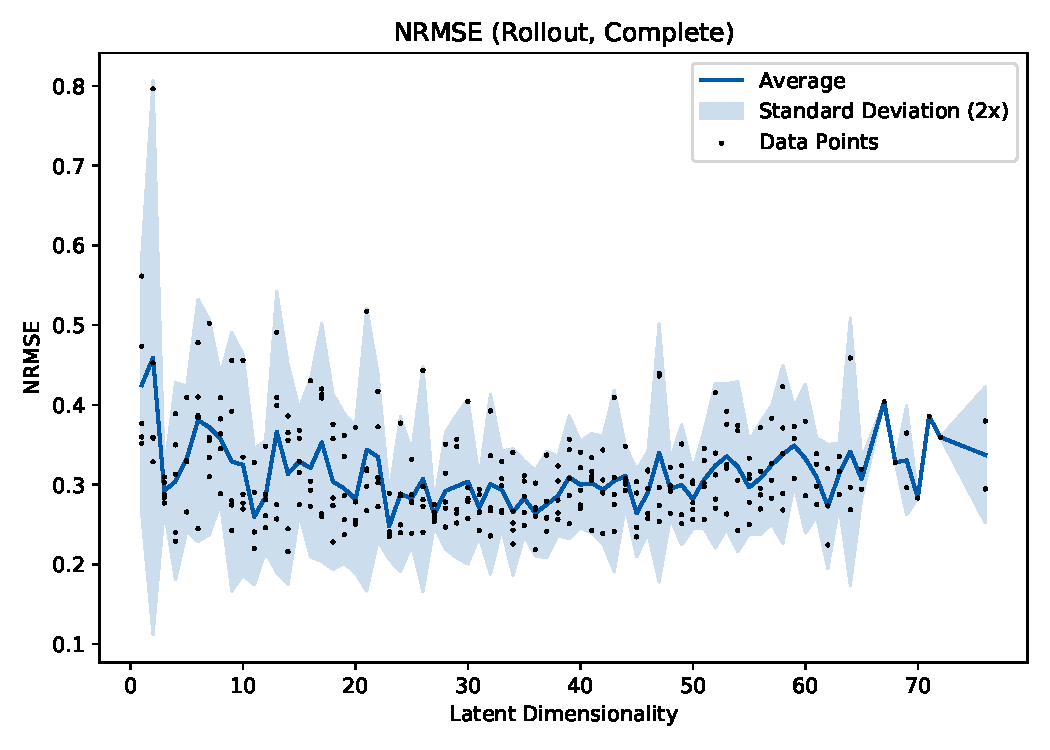
\includegraphics[width=\linewidth]{figures/results/cartpole-gym/latent-dim/comparison-rmse-rollout-normalized-mean-vs-latent-dim.pdf}
					\caption{Error of the complete rollout from on the cartpole environment.}
					\label{fig:cartpoleRmseComplete}
				\end{subfigure} \\
				\begin{subfigure}{0.5\linewidth}
					\centering
					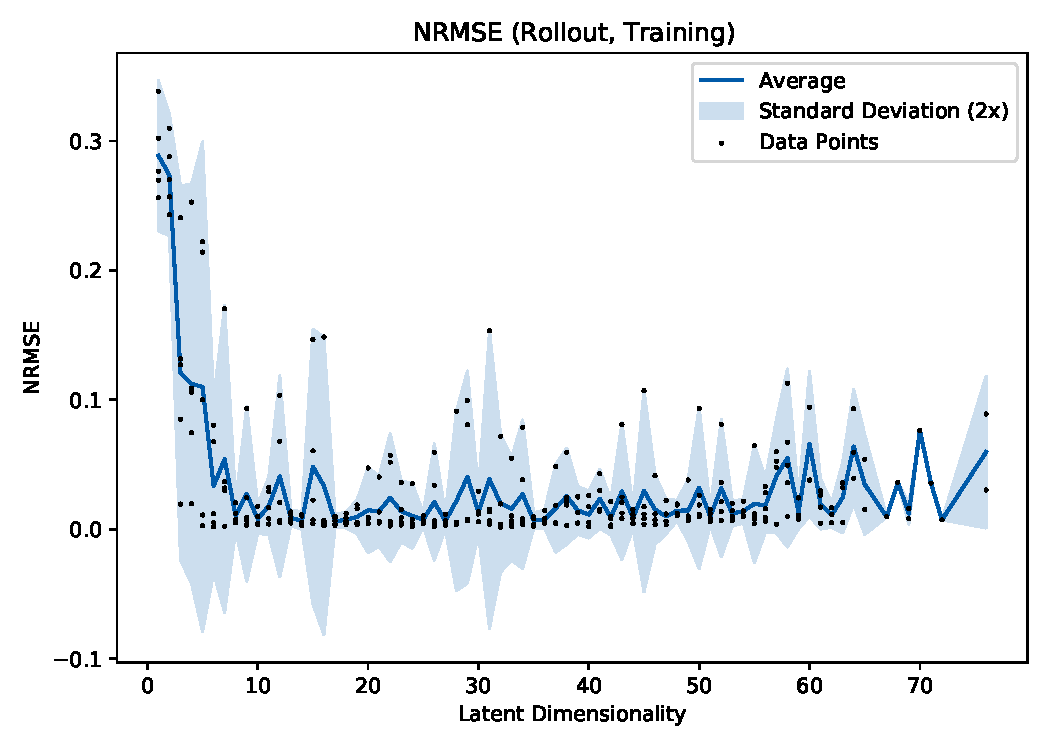
\includegraphics[width=\linewidth]{figures/results/cartpole-gym/latent-dim/comparison-rmse-rollout-train-normalized-mean-vs-latent-dim.pdf}
					\caption{Error of the rollout on the training data only on the cartpole environment.}
					\label{fig:cartpoleRmseTrain}
				\end{subfigure}%
				~
				\begin{subfigure}{0.5\linewidth}
					\centering
					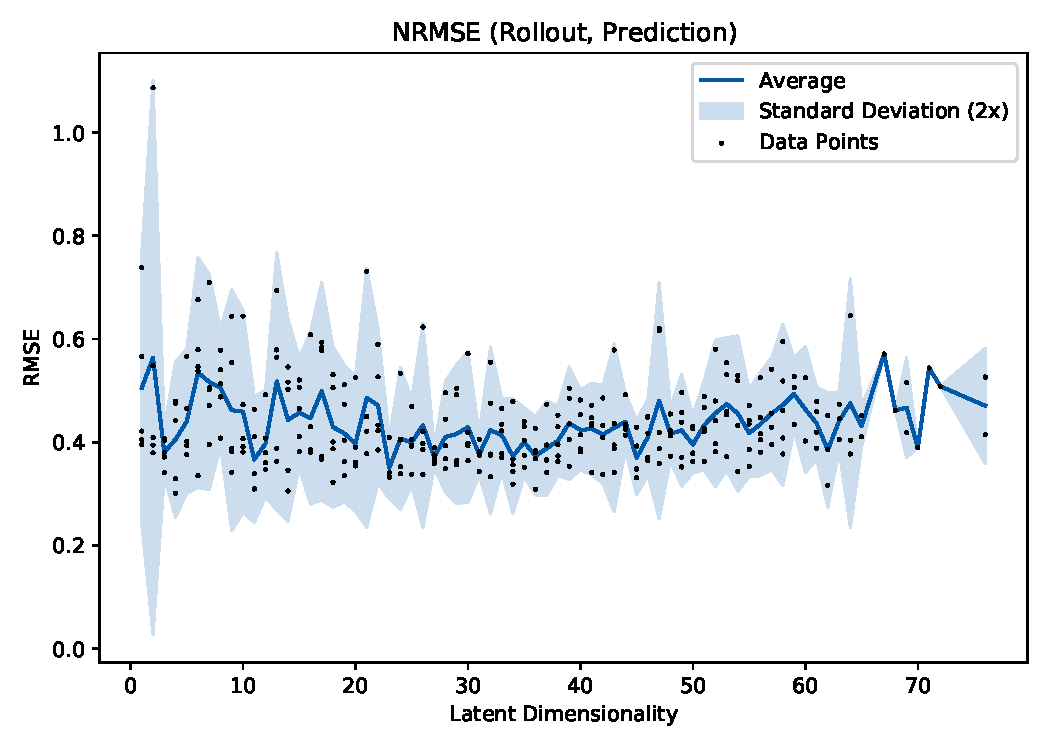
\includegraphics[width=\linewidth]{figures/results/cartpole-gym/latent-dim/comparison-rmse-rollout-prediction-normalized-mean-vs-latent-dim.pdf}
					\caption{Error of the rollout on the prediction only on the cartpole environment.}
					\label{fig:cartpoleRmsePred}
				\end{subfigure}
				\caption{Plot of the errors of the cartpole environment for different latent dimensions. The black dots show the measured data, the blue line the average of the data points at a specific time step. The blue shaded region shows two times the standard deviation. The data points on the right side of the plot get increasingly sparse as the algorithm gets increasingly numerically brittle for higher latent dimensionalities.}
				\label{fig:cartpoleRmse}
			\end{figure}
		% end

		\subsubsection{Exemplary Evaluation: 2-Dimensional Latent}
			We will now look at an exemplary run for the latent dimensionality \( k = 2 \) (run \texttt{356}). As we have already seen, the rollout should not perform well, but the smoothed trajectory should be really accurate. Looking at~\autoref{fig:cartpoleRolloutL02}, we see that nearly all trajectories are far off the true trajectory. Only the smoothed trajectory fits the data perfectly (until the prediction boundary, of course).

			\begin{figure}
				\centering
				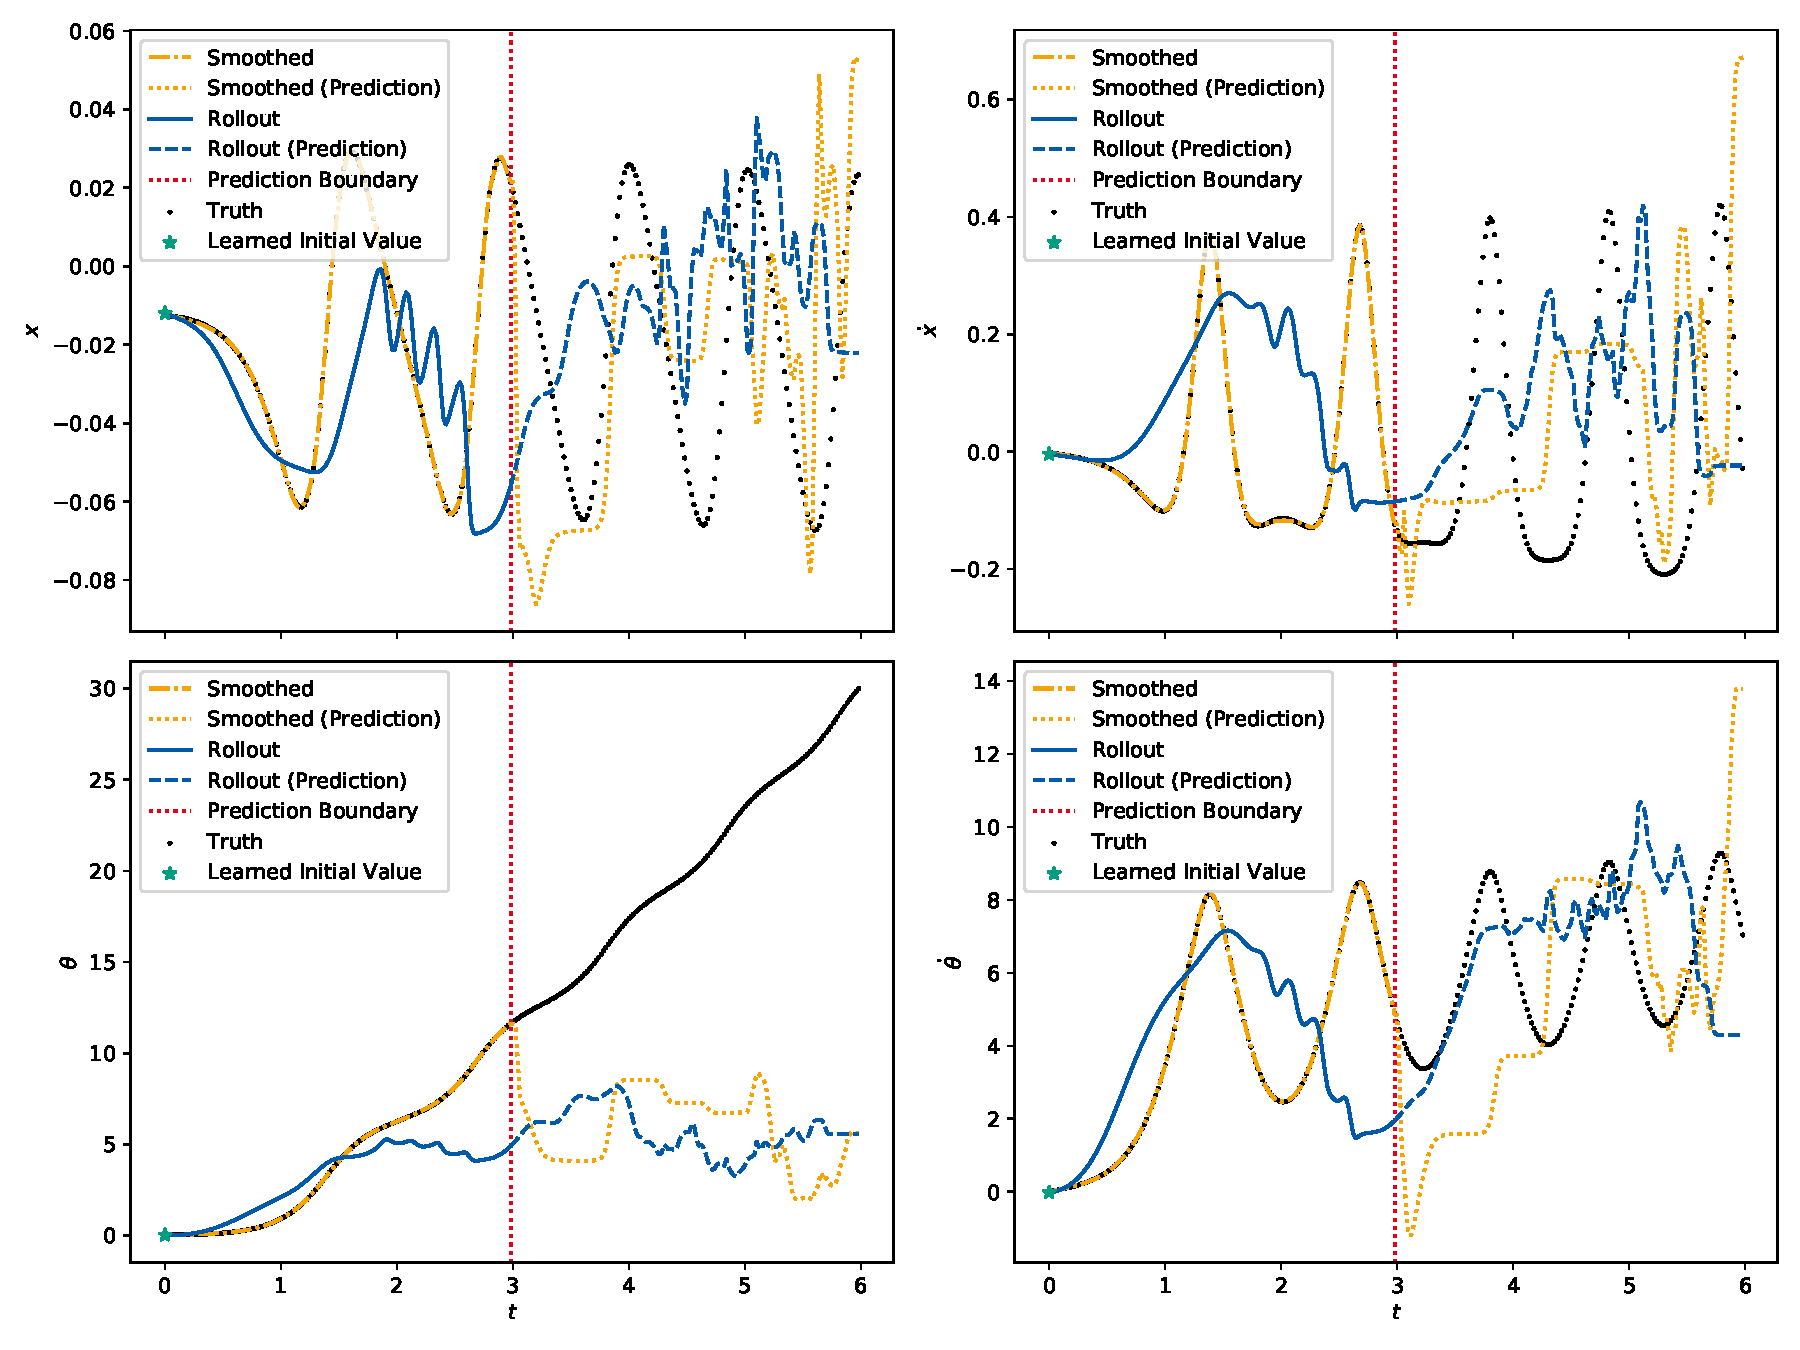
\includegraphics[width=\linewidth]{figures/results/cartpole-gym/run-latent-dim-02/without-confidence/rollout-observations-N0.pdf}
				\caption{The rollout plot in the observation space of the cartpole environment for \(k = 2\). The top plot is the cart position (left) and velocity (right), the row the pole displacement (left) and angular velocity (right). The black dots represent the true data of which the model used everything till the red prediction boundary to train on. The blue line is the rollout, starting from the learned initial value (marked with a green star). The orange dash-dotted line is the smoothed data. The dotted orange line then is the rollout starting from the last smoothed state, forming the "smoothed prediction". Note that we have removed the confidence on this plot as it is really low, result in high variances. See~\autoref{fig:cartpoleRolloutL02Appendix} in~\autoref{app:remainingPlots} for the plot with confidence.}
				\label{fig:cartpoleRolloutL02}
			\end{figure}
		% end

		\subsubsection{Exemplary Evaluation: 10-Dimensional Latent}
			We will now look at an exemplary run for the latent dimensionality \( k = 10 \) (run \texttt{462}). According to the \ac{nrmse} of the training data, this should perform decent on the training data and, according to the \ac{nrmse} on the prediction, bad on the prediction.~\autoref{fig:cartpoleRolloutL10} shows that the rollout and the smoothed trajectory actually follow the true data really good, while the rollout diverges from the true trajectory pretty fast after the prediction boundary. Also the variance in the training area around changes in the plot, \ac{ie} when the system actually moves or changes its velocity, is very high. Interestingly, the confidence in the pendulum position and velocity is a lot higher than in the cart position.

			\begin{figure}
				\centering
				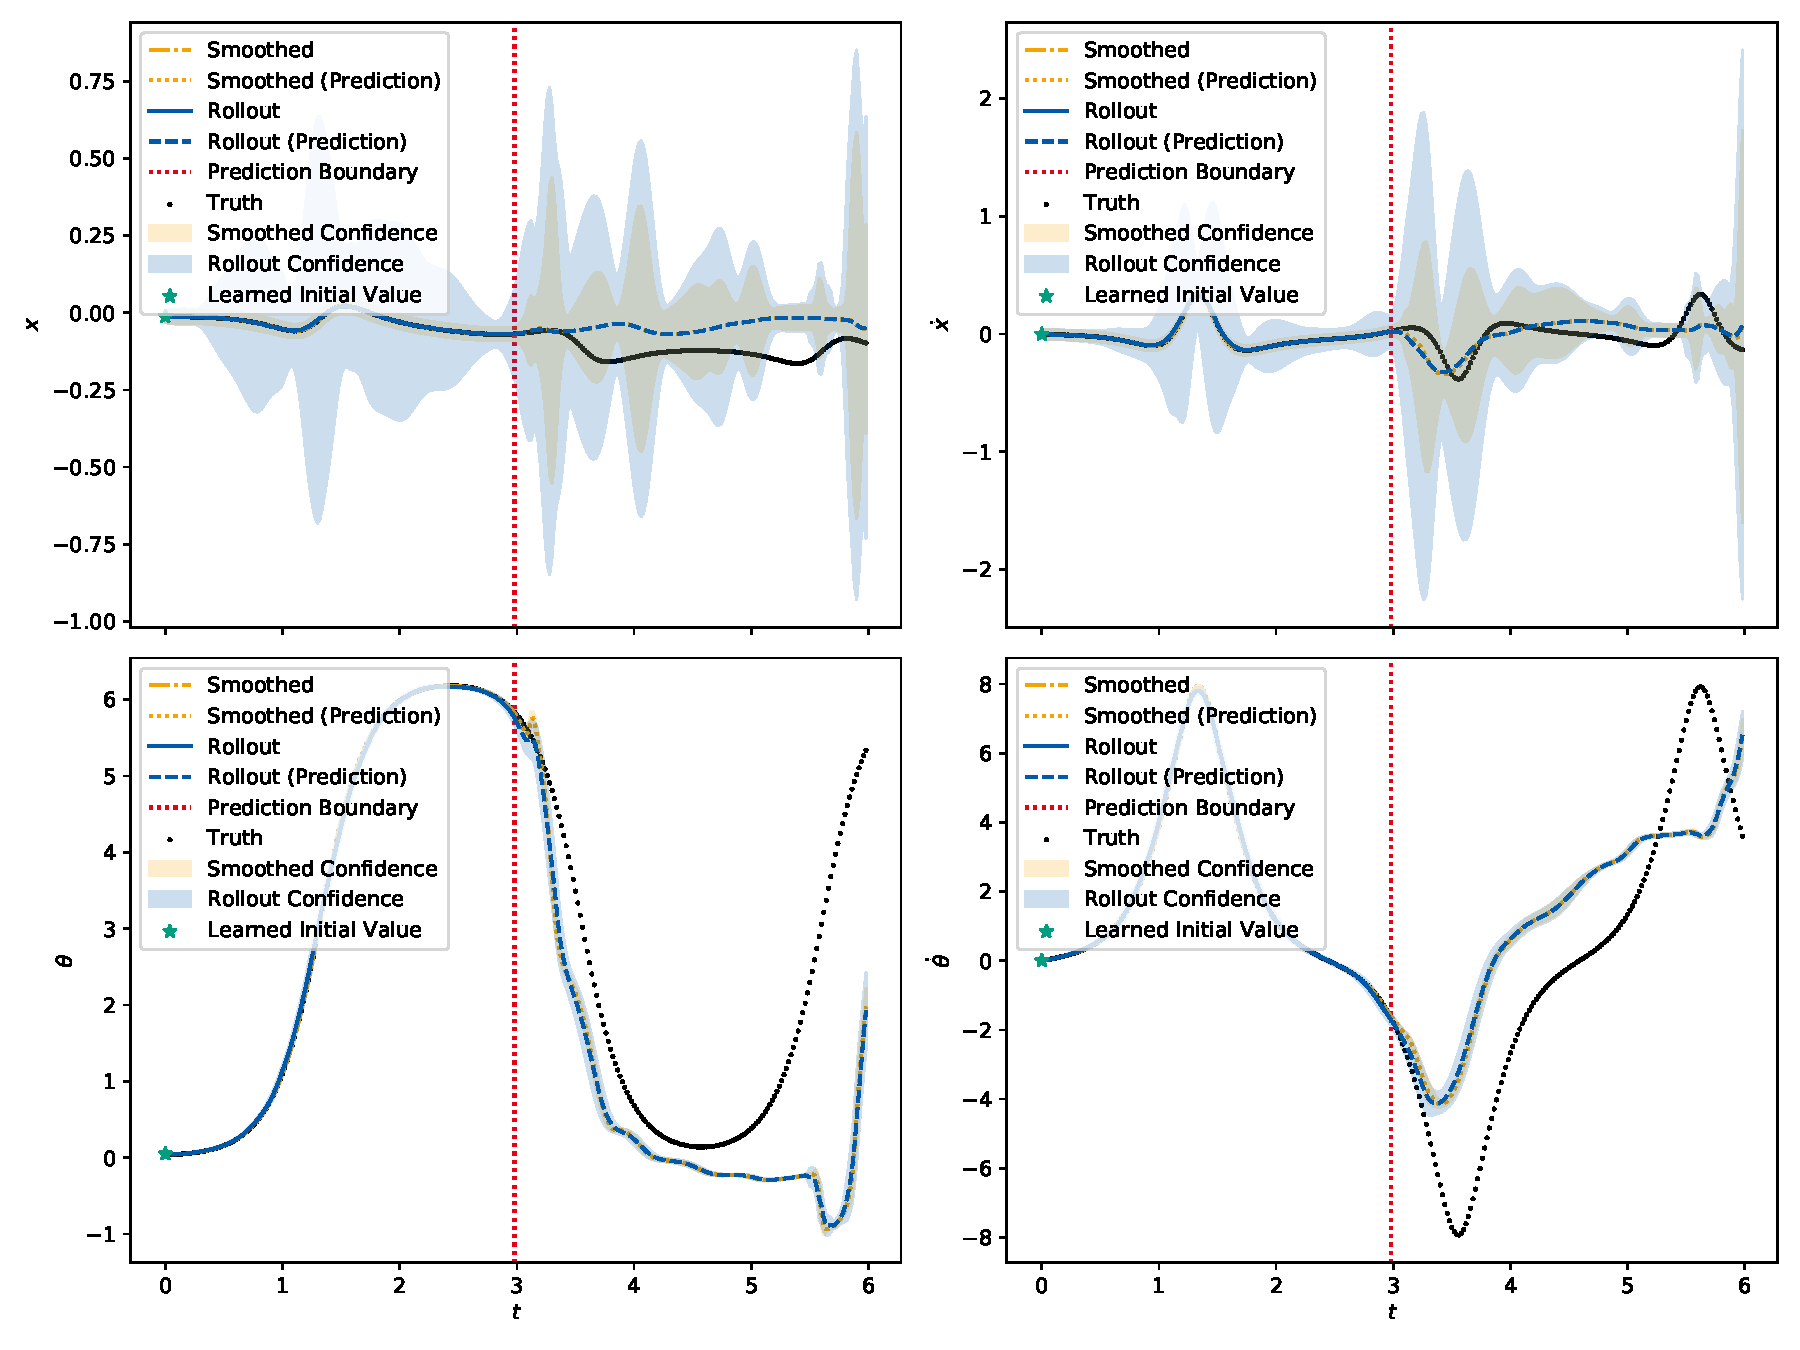
\includegraphics[width=\linewidth]{figures/results/cartpole-gym/run-latent-dim-10/rollout-observations-N0.pdf}
				\caption{The rollout plot in the observation space of the cartpole environment for \(k = 10\). The top plot is the cart position (left) and velocity (right), the row the pole displacement (left) and angular velocity (right). The black dots represent the true data of which the model used everything till the red prediction boundary to train on. The blue line is the rollout, starting from the learned initial value (marked with a green star). The orange dash-dotted line is the smoothed data. The dotted orange line then is the rollout starting from the last smoothed state, forming the "smoothed prediction". The shaded regions show the confidence, \ac{ie} two times the standard deviation. As the variances in the top plots are very high, see~\autoref{fig:cartpoleRolloutL10Appendix} in~\autoref{app:remainingPlots} for the plot without the confidence.}
				\label{fig:cartpoleRolloutL10}
			\end{figure}
		% end

		\subsubsection{Exemplary Evaluation: 14-Dimensional Latent}
			We will now look at an exemplary run for the latent dimensionality \( k = 14 \) (run \texttt{14}), the run which had the lowest \ac{nrmse} over the complete rollout data. Still, according to the \ac{nrmse} of the prediction, we do not expect a good prediction.~\autoref{fig:cartpoleRolloutL14} confirms this, as the rollout on the training data follows the true data closely while the prediction is off the true trajectory.

			\begin{figure}
				\centering
				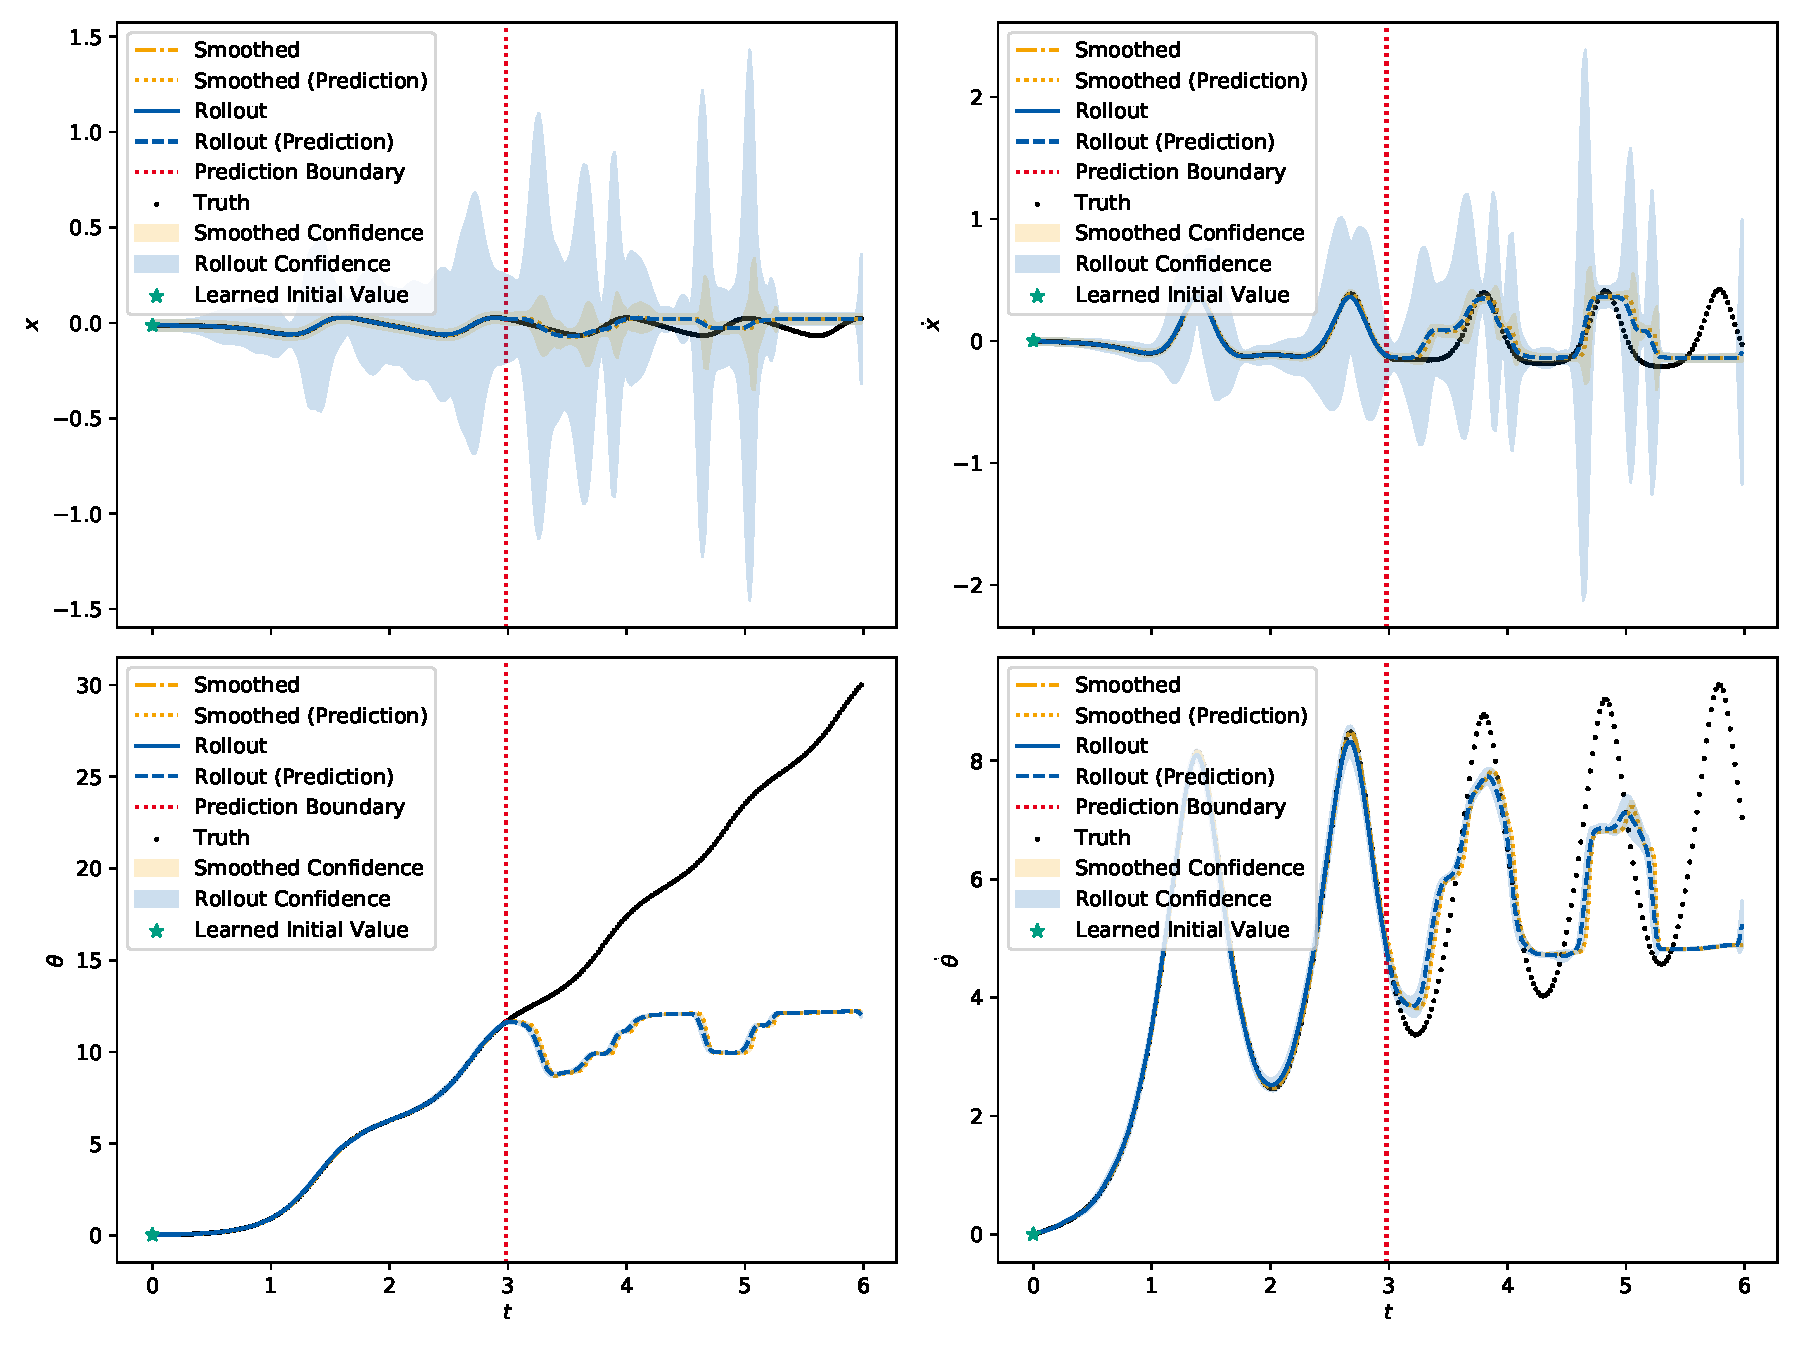
\includegraphics[width=\linewidth]{figures/results/cartpole-gym/run-latent-dim-14/rollout-observations-N0.pdf}
				\caption{The rollout plot in the observation space of the cartpole environment for \(k = 14\). The top plot is the cart position (left) and velocity (right), the row the pole displacement (left) and angular velocity (right). The black dots represent the true data of which the model used everything till the red prediction boundary to train on. The blue line is the rollout, starting from the learned initial value (marked with a green star). The orange dash-dotted line is the smoothed data. The dotted orange line then is the rollout starting from the last smoothed state, forming the "smoothed prediction". The shaded regions show the confidence, \ac{ie} two times the standard deviation. As the variances in the top plots are still very high, see~\autoref{fig:cartpoleRolloutL14Appendix} in~\autoref{app:remainingPlots} for the plot without the confidence.}
				\label{fig:cartpoleRolloutL14}
			\end{figure}
		% end
	% end

	\subsection{Gym Double Pendulum}
		\todo{Update with latest experiment! The experiment that ran on the GPU.}

		\subsubsection{Influence of the Latent Dimensionality}
			For the double pendulum experiment, we tested \(50\) latent dimensionalities from \( k = 1 \) to \( k = 50 \).

			We will start by having a first look at the \ac{nrmse} of the smoothed trajectory in~\autoref{fig:acrobotRmseSmoothed} to see how many latent dimensions we need the least to get a model that is even slightly capable of learning the double pendulum dynamics. We see that the \ac{nrmse} shrinks below \(0.05\) for latent dimensionalities of \( k \geq 3 \), so we need at least \(3\) latent dimensions to get a decent model.

			Looking at the \ac{nrmse} of the complete rollout in~\autoref{fig:acrobotRmseComplete}, we see that the error shrinks until \( k \geq 6 \) latent dimensions and than stabilizes to an error around \( 0.28 \), not shrinking much anymore (the error for \( k = 49 \) is approximately \( 0.24 \)). Looking at the training and prediction error in~\autoref{fig:acrobotRmseTrain} and~\autoref{fig:acrobotRmsePred}, we see that mostly only the training error shrinks while the prediction errors seems to random noise. Hence, we can assume that our model does not generalize well (we will assess this in~\autoref{c:discussion}). On the other hand, our rollout on the training data should be a good fit.

			\begin{figure}
				\centering
				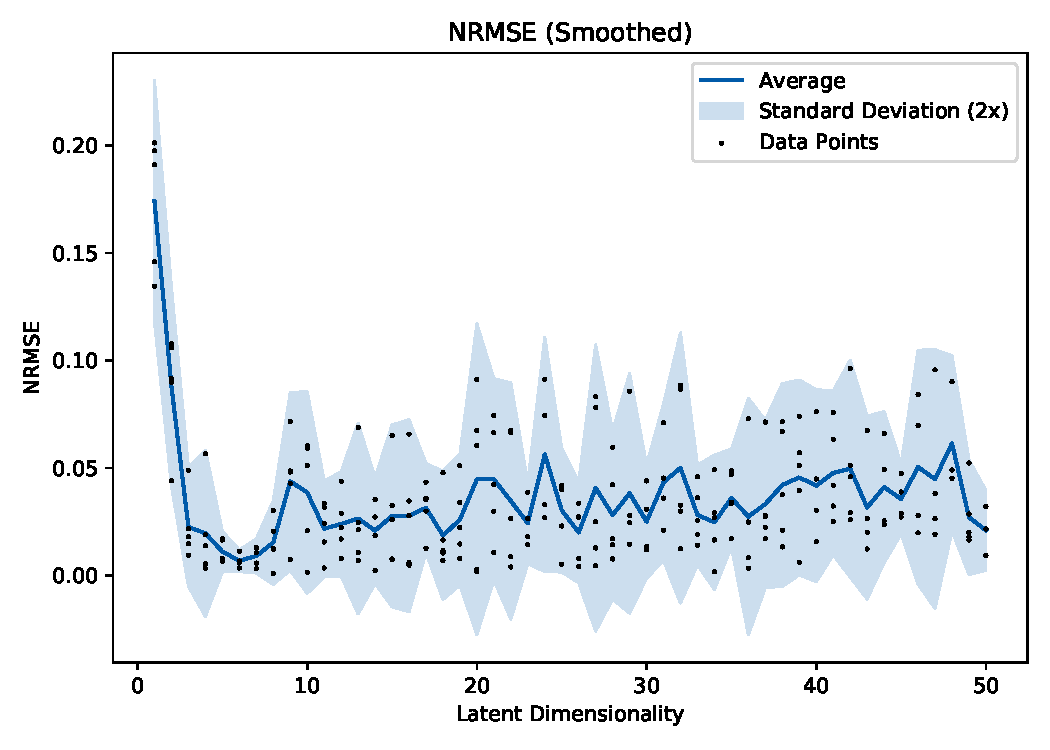
\includegraphics[width=0.7\linewidth]{figures/results/acrobot-gym/latent-dim/comparison-rmse-smoothed-normalized-mean-vs-latent-dim.pdf}
				\caption{The \ac{nrmse} of the smoothed trajectory on the training data of the double pendulum environment.}
				\label{fig:acrobotRmseSmoothed}
			\end{figure}

			\begin{figure}
				\centering
				\begin{subfigure}{0.7\linewidth}
					\centering
					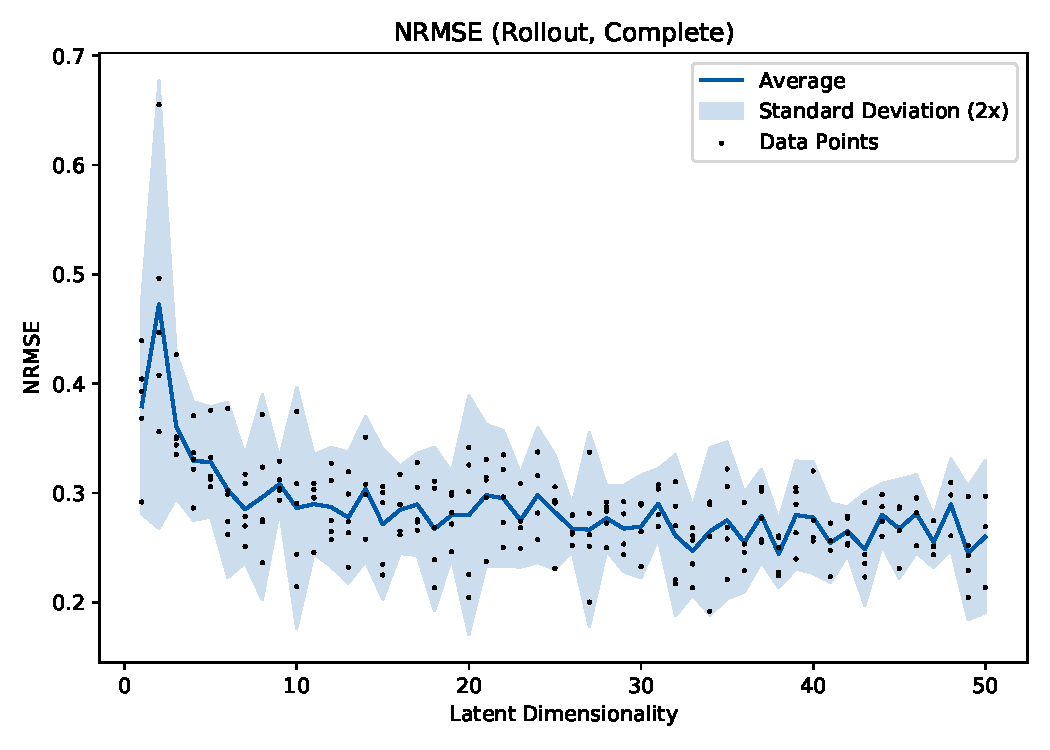
\includegraphics[width=\linewidth]{figures/results/acrobot-gym/latent-dim/comparison-rmse-rollout-normalized-mean-vs-latent-dim.pdf}
					\caption{Error of the complete rollout from on the cartpole double pendulum.}
					\label{fig:acrobotRmseComplete}
				\end{subfigure} \\
				\begin{subfigure}{0.5\linewidth}
					\centering
					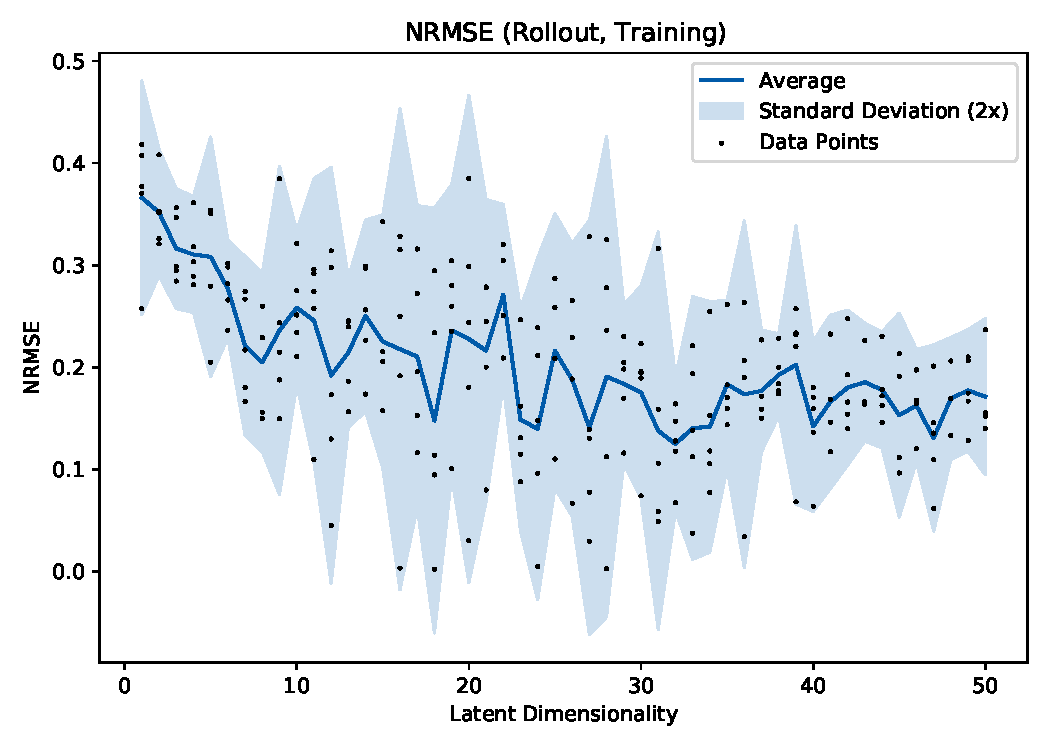
\includegraphics[width=\linewidth]{figures/results/acrobot-gym/latent-dim/comparison-rmse-rollout-train-normalized-mean-vs-latent-dim.pdf}
					\caption{Error of the rollout on the training data only on the double pendulum environment.}
					\label{fig:acrobotRmseTrain}
				\end{subfigure}%
				~
				\begin{subfigure}{0.5\linewidth}
					\centering
					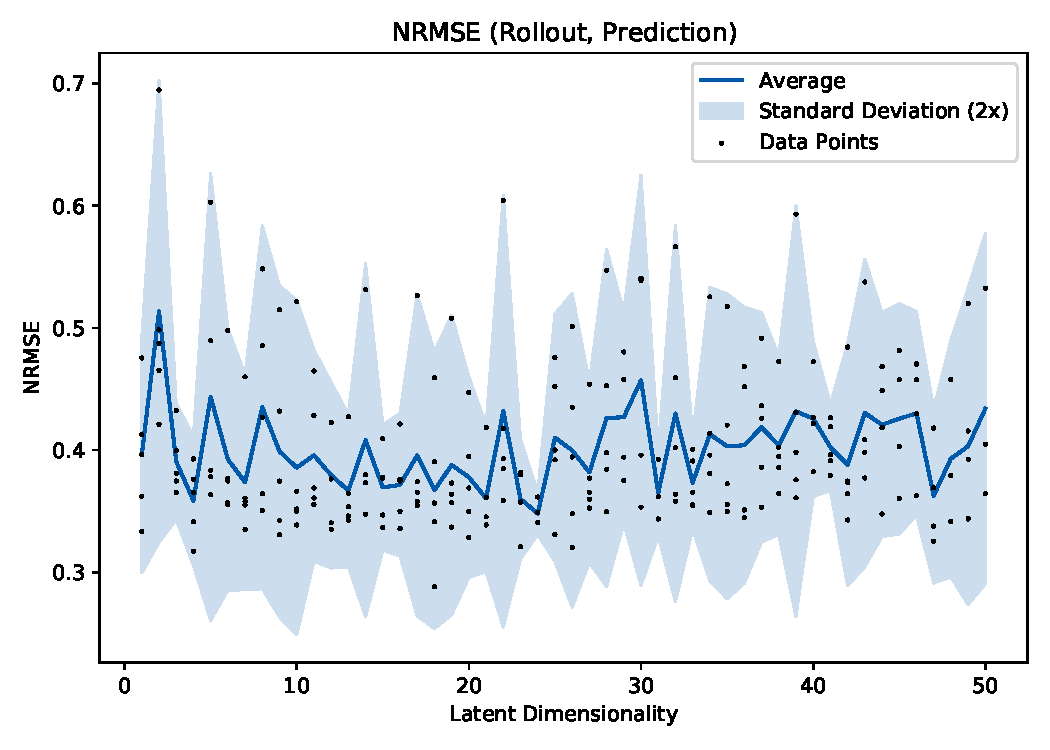
\includegraphics[width=\linewidth]{figures/results/acrobot-gym/latent-dim/comparison-rmse-rollout-prediction-normalized-mean-vs-latent-dim.pdf}
					\caption{Error of the rollout on the prediction only on the double pendulum environment.}
					\label{fig:acrobotRmsePred}
				\end{subfigure}
				\caption{Plot of the errors of the double pendulum environment for different latent dimensions. The black dots show the measured data, the blue line the average of the data points at a specific time step. The blue shaded region shows two times the standard deviation. The data points on the right side of the plot get increasingly sparse as the algorithm gets increasingly numerically brittle for higher latent dimensionalities.}
				\label{fig:acrobotRmse}
			\end{figure}
		% end

		\subsubsection{Exemplary Evaluation: 3-Dimensional Latent}
			We will now look at an exemplary run for the latent dimensionality \( k = 3 \) (run \texttt{103}). As we have already seen, the rollout should not perform well, but the smoothed trajectory should be really accurate. Looking at~\autoref{fig:acrobotRolloutL03}, we see that nearly all trajectories are far off the true trajectory. Only the smoothed trajectory follows the data decently (until the prediction boundary, of course).

			\begin{figure}
				\centering
				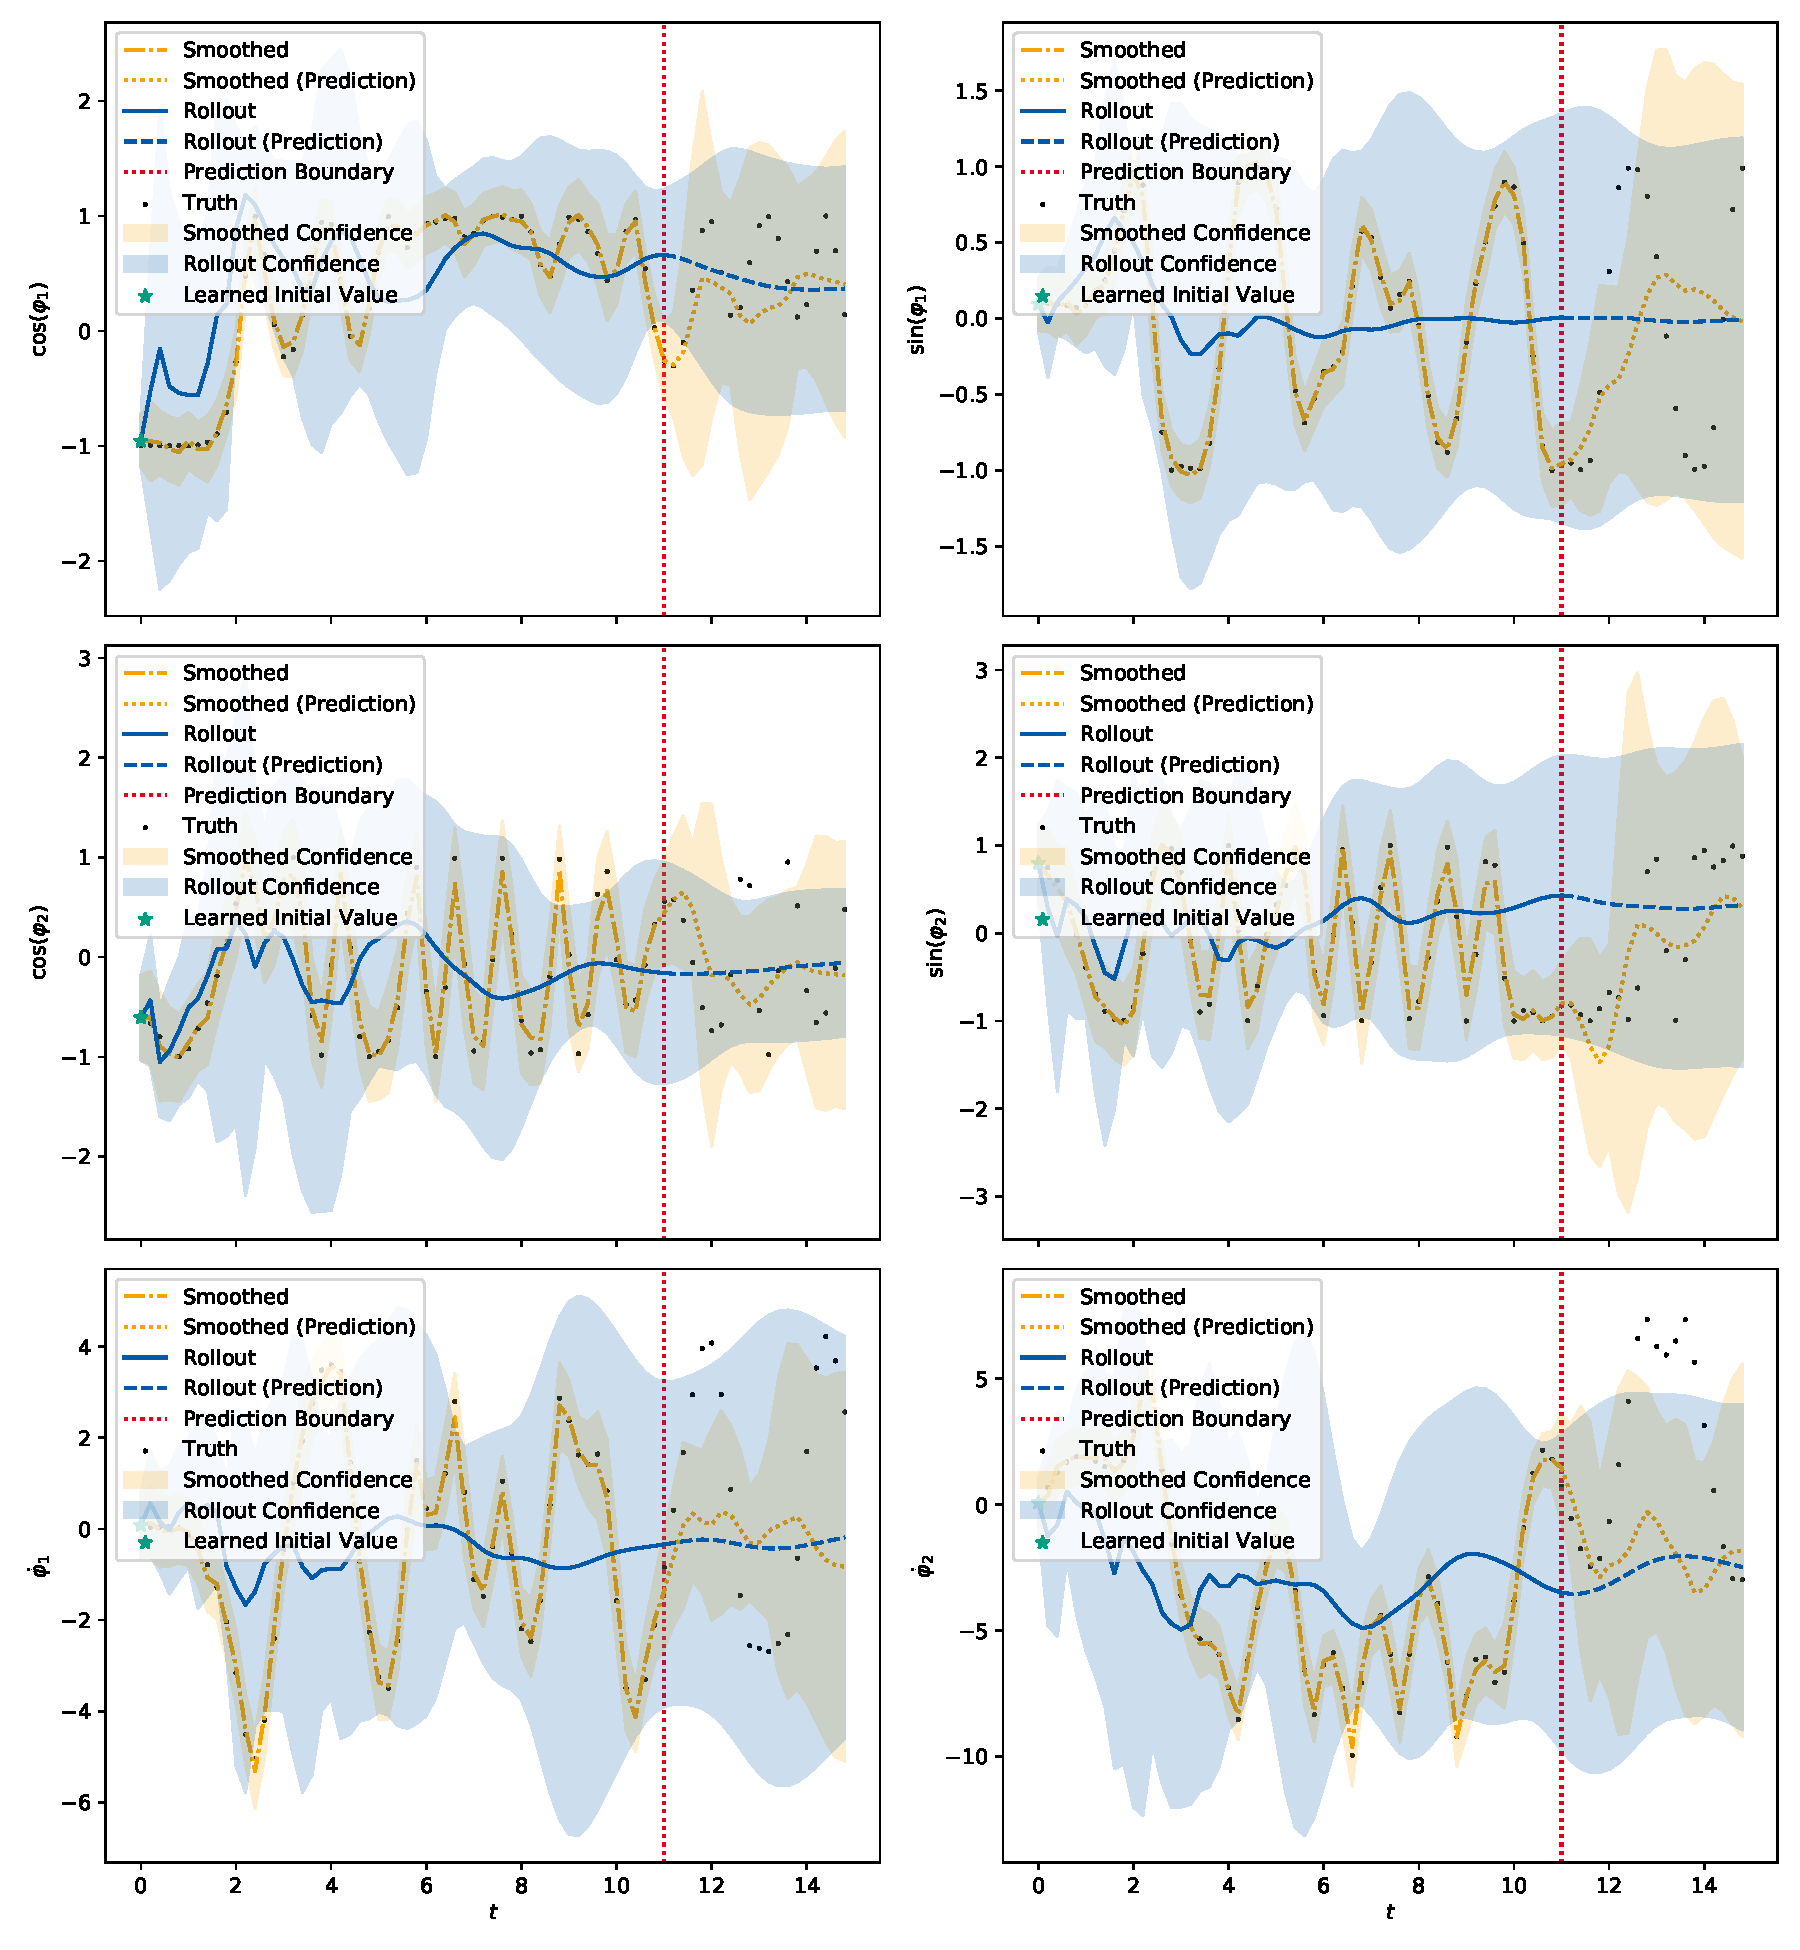
\includegraphics[width=\linewidth]{figures/results/acrobot-gym/run-latent-dim-03/rollout-observations-N0.pdf}
				\caption{The rollout plot in the observation space of the double pendulum environment for \(k = 3\). The top row shows the cosine/sine of the displacement of the inner pendulum, the middle row shows the cosine/sine of the displacement of the outer pendulum and the bottom row shows the angular velocity of the inner and outer pendulum. The black dots represent the true data of which the model used everything till the red prediction boundary to train on. The blue line is the rollout, starting from the learned initial value (marked with a green star). The orange dash-dotted line is the smoothed data. The dotted orange line then is the rollout starting from the last smoothed state, forming the "smoothed prediction". The shaded regions show the confidence, \ac{ie} two times the standard deviation.}
				\label{fig:acrobotRolloutL03}
			\end{figure}
		% end

		\subsubsection{Exemplary Evaluation: 6-Dimensional Latent}
			% TODO
		% end

		\subsubsection{Exemplary Evaluation: 34-Dimensional Latent}
			% TODO
		% end
	% end
% end
